\documentclass[11pt,a4paper]{article}

\usepackage[margin=3cm]{geometry}
\usepackage{amsmath,amssymb,amsthm}
\usepackage{mathtools}
\usepackage{microtype}
\usepackage{xcolor}
\usepackage{tikz}
\usepackage[british]{babel}
\usepackage[hidelinks]{hyperref}
\usepackage[capitalise,noabbrev]{cleveref}

\theoremstyle{plain}
\newtheorem{theorem}{Theorem}
\newtheorem*{theorem*}{Theorem}
\newtheorem{proposition}[theorem]{Proposition}
\newtheorem{corollary}[theorem]{Corollary}
\newtheorem{lemma}[theorem]{Lemma}
\theoremstyle{definition}
\newtheorem{remark}[theorem]{Remark}

\AddToHook{env/theorem/begin}{\crefalias{theorem}{theorem}}
\AddToHook{env/proposition/begin}{\crefalias{theorem}{proposition}}
\AddToHook{env/corollary/begin}{\crefalias{theorem}{corollary}}
\AddToHook{env/lemma/begin}{\crefalias{theorem}{lemma}}
\AddToHook{env/remark/begin}{\crefalias{theorem}{remark}}

\DeclareMathOperator{\CFI}{CFI}
\DeclareMathOperator{\tr}{tr}
\DeclareMathOperator{\val}{val}
\DeclareMathOperator{\supp}{supp}
\DeclareMathOperator{\rank}{rank}
\DeclareMathOperator{\diag}{diag}
\DeclareMathOperator{\spn}{span}
\DeclareMathOperator{\im}{im}
\DeclareMathOperator{\len}{len}

\newcommand{\R}{\mathbb{R}}
\newcommand{\Z}{\mathbb{Z}}
\newcommand{\calF}{\mathcal{F}}
\newcommand{\ones}{\mathbf{1}}

\title{Distinguishing graphs with simple spectrum\\by homomorphism counts}
\author{Takanori Maehara\thanks{\texttt{tmaehara@acm.org}}}
\date{29 September 2026}
\hypersetup{
  pdftitle={Distinguishing graphs with simple spectrum by homomorphism counts},
  pdfauthor={Takanori Maehara}
}

\begin{document}
\maketitle
\begin{abstract}
We study which graph classes determine every graph with simple spectrum
up to isomorphism by homomorphism counts from their members.
We show that such a class has unbounded treewidth and Euler genus and
contains a graph with the complete graph on seven vertices as a minor.
To prove these conditions, we construct pairs of non-isomorphic cospectral
graphs with simple spectrum, each bipartite, nonsingular and of maximum
degree at most six.
The construction attaches rooted trees to Cai--F\"urer--Immerman graphs and
preserves homomorphism indistinguishability over every minor-closed class.
We then prove that subcubic homomorphism counts determine every graph whose
adjacency matrix has kernel dimension at most one.
This extends the known result for nonsingular graphs and applies to all
graphs with simple spectrum.
We also prove that two graphs have the same subcubic homomorphism counts
if and only if they have the same number of vertices and there is a
bijective linear isometry between the images of their adjacency matrices
that intertwines the adjacency operators and preserves the coordinatewise
trilinear forms.
Finally, we prove that homomorphism counts from the single-vertex graph
and from subdivisions of any sequence of connected cubic graphs have
the same distinguishing power as subcubic homomorphism counts if every
complete graph is a minor of some member of the sequence.
\end{abstract}

{\small
\noindent\textbf{Keywords.}
graph homomorphism, graph isomorphism, graph spectrum.
\par\smallskip
\noindent\textbf{2020 Mathematics Subject Classification.}
05C60, 05C50, 05C83.
\par}

\section{Introduction and Main Results}
\label{sec:intro}

Graphs are finite, simple and undirected unless stated otherwise.
We write $N_G(x)$ for the set of neighbours of $x$ in $G$ and
$\R^\times=\R\setminus\{0\}$ for the set of nonzero real numbers.
The \emph{nullity} of a graph is the dimension of the kernel of its
adjacency matrix.
A \emph{homomorphism} from a graph $F$ to a graph $G$
is a map from $V(F)$ to $V(G)$ that preserves adjacency. We write
$\hom(F,G)$ for the number of such maps. Two graphs $G$ and $G'$ are \emph{homomorphism
indistinguishable} over a graph class $\mathcal C$, written
$G\equiv_{\mathcal C}G'$, if
$\hom(F,G)=\hom(F,G')$ for every $F\in\mathcal C$.

Homomorphism counts characterise a range of graph properties and
equivalence relations. Lov\'asz~\cite{Lovasz1967} proved that two graphs
$G$ and $G'$ are isomorphic if and only if $\hom(F,G)=\hom(F,G')$ for every
graph $F$.
A graph is bipartite if and only if its homomorphism count from every odd
cycle is zero. Two graphs $G$ and $G'$ with the same number of vertices
are cospectral if and only if $\hom(C,G)=\hom(C,G')$ for every cycle $C$,
because the homomorphism count from the $k$-cycle to a graph is the trace
of the $k$-th power of its adjacency matrix. For every $k\geq1$, two graphs are
homomorphism indistinguishable over the graphs of treewidth at most $k$ if
and only if the $k$-dimensional Weisfeiler--Leman test does not distinguish
them~\cite{Dvorak2010,DellGroheRattan2018}.

A graph has \emph{simple spectrum} if its adjacency matrix has pairwise
distinct eigenvalues. We study homomorphism characterisations of
isomorphism on graphs with simple spectrum.
We call a class \emph{complete on simple spectrum} if any two graphs with
simple spectrum that are homomorphism indistinguishable over the class
are isomorphic.
By the result of Lov\'asz, the class of all graphs is complete on simple
spectrum. Since isomorphism testing on graphs with simple spectrum is
possible in polynomial time~\cite{BabaiGrigoryevMount1982}, we ask which
smaller classes are still complete on simple spectrum.

We first prove that the following graph classes are not complete on
simple spectrum.

\begin{theorem}\label{thm:incompleteness}
Let $\mathcal C$ be any one of the following graph classes:
\begin{enumerate}
 \item graphs of treewidth at most $k$, for a fixed integer $k\geq1$;
 \item graphs embeddable on a surface of Euler genus at most $g$, for a fixed integer $g\geq0$;
 \item graphs with no $K_7$ minor.
\end{enumerate}
There are non-isomorphic graphs $G,G'$ with simple spectrum such that
$G\equiv_{\mathcal C}G'$.
The graphs $G$ and $G'$ can be chosen cospectral with each other, with
each of them bipartite, nonsingular, and of maximum degree at most six.
Consequently every class complete on simple spectrum has unbounded treewidth
and unbounded Euler genus, and contains a graph with a $K_7$ minor.
\end{theorem}

The first case of \cref{thm:incompleteness} answers the question of Hordan, Dym and
Seppelt~\cite[Section~7]{HordanDymSeppelt2026}, who proved this
incompleteness for multigraphs and asked whether it holds for simple graphs.
The second case with $g=0$ covers planar graphs. Planar graphs have
unbounded treewidth, so unbounded treewidth alone does not suffice for
completeness.
The proof attaches rooted trees to a pair of Cai--F\"urer--Immerman graphs.
The two resulting graphs have simple spectrum and are homomorphism
indistinguishable over every minor-closed class over which the original pair
is homomorphism indistinguishable
(\cref{lem:ss-transfer}).
The two Cai--F\"urer--Immerman graphs are homomorphism indistinguishable
from each other over each of the three classes by known results.

It remains open whether every class complete on simple spectrum must contain
graphs with arbitrarily large clique minors. An affirmative answer would
imply the weak Roberson conjecture, which states that for every proper
minor-closed graph class there are two non-isomorphic graphs that are
homomorphism indistinguishable over the
class~\cite[Conjecture~5 and Theorem~8.4]{Roberson2026};
see \cref{rem:ss-minor-necessity}.

We next ask which graph classes suffice for completeness on simple
spectrum. A graph is \emph{subcubic} if its maximum degree is at most
three. Let $\mathcal D_3$ be the class of subcubic graphs.
There are non-isomorphic graphs that are homomorphism indistinguishable
over $\mathcal D_3$~\cite{Roberson2026}. Our next result shows that
subcubic homomorphism counts nevertheless determine every graph of nullity
at most one up to isomorphism. A graph with simple spectrum has nullity at
most one, so the result covers every graph with simple spectrum.

\begin{theorem}\label{thm:main}
 Let $G$ be a graph of nullity at most one. For every graph $G'$,
 $G\equiv_{\mathcal D_3}G'$ if and only if $G\cong G'$.
 In particular, $\mathcal D_3$ is complete on simple spectrum.
\end{theorem}

\Cref{thm:main} extends~\cite[Corollary~38]{CaiYoung2026} from
nonsingular graphs to graphs of nullity at most one.
\Cref{lem:characterisation} characterises subcubic homomorphism
indistinguishability for arbitrary graphs $G,G'$:
$G\equiv_{\mathcal D_3}G'$ if and only if
$G$ and $G'$ have the same number of vertices and there is a bijective
linear isometry between the images of their adjacency matrices that
intertwines the adjacency operators and preserves the coordinatewise
trilinear forms.
For degree bound three, \cref{lem:characterisation} is the more specific
characterisation suggested after Corollary~39 of~\cite{CaiYoung2026}.

It remains open whether \cref{thm:main} extends to nullity two, but there
are counterexamples of nullity three; see \cref{rem:nullity-bound}.

Finally, we show that homomorphism counts from subdivisions of suitable
cubic graphs, together with the number of vertices, have the same
distinguishing power as counts from all subcubic graphs.
\begin{proposition}\label{prop:closure}
 Let $(H_N)_{N\geq1}$ be a sequence of connected cubic graphs such that,
 for every $t\geq1$, some $H_N$ contains $K_t$ as a minor.
 Let $\calF$ consist of $K_1$ and all subdivisions of the graphs $H_N$.
 Then
 \begin{equation}\label{eq:restriction-equivalence}
  G\equiv_{\calF}G'\Longleftrightarrow
  G\equiv_{\mathcal D_3}G'
 \end{equation}
 for all graphs $G,G'$. In particular, $\calF$ is complete on simple spectrum.
\end{proposition}
Including $K_1$ in $\calF$ is necessary: $K_2$ and $K_2\sqcup K_1$ have simple
spectrum and equal homomorphism counts from every connected graph with at least two vertices.

\section{Proof of Theorem~\ref{thm:incompleteness}}
\label{sec:incompleteness}

We use the variant of the Cai--F\"urer--Immerman (CFI)
construction~\cite{CaiFurerImmerman1992} given
in~\cite[Definition~3.1]{Roberson2026}.
Let $B$ be a connected graph and $v_*$ a vertex of $B$.
For a vertex $v$ of $B$, the set of edges incident with $v$ is denoted by
$E_B(v)$.
For $i\in\{0,1\}$, let $\CFI_i(B)$ be the graph with
\begin{equation}\label{eq:ss-cfi-definition}
 \begin{aligned}
 \Xi_i(v)&=\left\{\xi\in\mathbb F_2^{E_B(v)}:
   \sum_{e\in E_B(v)}\xi_e=i\delta_{v,v_*}\right\},\\
 V(\CFI_i(B))&=\{(v,\xi):v\in V(B),\xi\in \Xi_i(v)\},\\
 E(\CFI_i(B))&=\{(v,\xi)(w,\zeta):vw\in E(B),\xi\in \Xi_i(v),\zeta\in \Xi_i(w),\xi_{vw}=\zeta_{vw}\}.
 \end{aligned}
\end{equation}
Here $\delta_{ab}$ is $1$ when $a=b$ and $0$ otherwise.
The vertices $(v,\xi)$ with $\xi\in \Xi_i(v)$ form a \emph{fibre} with
\emph{base vertex} $v$, and they are said to lie \emph{over} $v$.
The isomorphism type of $\CFI_1(B)$ is independent of the choice of
$v_*$, and the graphs $\CFI_0(B)$ and $\CFI_1(B)$ are non-isomorphic;
both facts follow from \cite[Lemma~5]{Neuen2024}.

For $i\in\{0,1\}$, let $\pi_i:\CFI_i(B)\to B$ be the projection
$\pi_i(v,\xi)=v$.
Let $F$ be a graph and $\chi:F\to B$ a homomorphism.
A homomorphism $f:F\to\CFI_i(B)$ is a \emph{lift} of $\chi$ if
$\pi_i\circ f=\chi$.
The number of such lifts is denoted by $\hom_\chi(F,\CFI_i(B))$.
We show that if $\hom(F,\CFI_0(B))=\hom(F,\CFI_1(B))$, then
$\hom_\chi(F,\CFI_0(B))=\hom_\chi(F,\CFI_1(B))$ for every homomorphism
$\chi:F\to B$.
For every fixed $\chi$, \cite[Theorem~3.6]{Roberson2026} gives
\begin{equation}\label{eq:ss-coloured-monotonicity}
  \hom_\chi(F,\CFI_1(B))\leq\hom_\chi(F,\CFI_0(B)).
\end{equation}
Every homomorphism $f:F\to\CFI_i(B)$ is a lift of exactly one map
$\chi=\pi_i\circ f$, so
\begin{equation}\label{eq:ss-lift-differences}
 \hom(F,\CFI_0(B))-\hom(F,\CFI_1(B))
 =\sum_\chi\bigl(\hom_\chi(F,\CFI_0(B))-\hom_\chi(F,\CFI_1(B))\bigr)
\end{equation}
is a sum of nonnegative terms. If the total counts agree, every term
therefore vanishes.
Consequently, for every graph $F$ and every homomorphism
$\chi:F\to B$,
\begin{equation}\label{eq:ss-lift-equality}
 \hom(F,\CFI_0(B))=\hom(F,\CFI_1(B))
 \Longrightarrow
 \hom_\chi(F,\CFI_0(B))=\hom_\chi(F,\CFI_1(B)).
\end{equation}

For a minor-closed class $\mathcal C$, the following lemma constructs
non-isomorphic graphs $G\equiv_{\mathcal C}G'$ with simple spectrum
whenever $\CFI_0(B)\equiv_{\mathcal C}\CFI_1(B)$.

\begin{lemma}\label{lem:ss-transfer}
Let $\mathcal C$ be a minor-closed graph class and let $B$ be a connected
graph satisfying $\CFI_0(B)\equiv_{\mathcal C}\CFI_1(B)$. Then there are non-isomorphic
graphs $G,G'$ with simple spectrum and $G\equiv_{\mathcal C}G'$.
The witnesses can be chosen bipartite, cospectral, nonsingular, and of
maximum degree at most six.
\end{lemma}

\begin{proof}[Proof of \cref{thm:incompleteness}]
By \cref{lem:ss-transfer}, it suffices to give, for each of the three
classes $\mathcal C$, a connected graph $B$ with
$\CFI_0(B)\equiv_{\mathcal C}\CFI_1(B)$.
When $\mathcal C$ is the class of graphs of treewidth at most $k\geq1$, the graph
$B=K_{k+2}$ satisfies
$\CFI_0(B)\equiv_{\mathcal C}\CFI_1(B)$~\cite[Theorem~10 and Lemma~12]{Neuen2024}.
When $\mathcal C$ is the class of graphs of Euler genus at most $g$, a connected
graph $B$ with $\CFI_0(B)\equiv_{\mathcal C}\CFI_1(B)$ is given in
\cite[Lemma~2.10 and proof of Theorem~1.8]{NeuenSeppelt2026}.
When $\mathcal C$ is the class of $K_7$-minor-free graphs, a connected graph $B$ with
$\CFI_0(B)\equiv_{\mathcal C}\CFI_1(B)$ is given in
\cite[Lemma~2.10 and proof of Theorem~1.9]{NeuenSeppelt2026}
and \cite[Theorem~1.7 and Section~1.3]{ThilikosWiederrecht2024}.
\end{proof}

The proof of \cref{lem:ss-transfer} has two steps.
If $\CFI_0(B)\equiv_{\mathcal C}\CFI_1(B)$ for a minor-closed class
$\mathcal C$, then the two graphs obtained from $\CFI_0(B)$ and
$\CFI_1(B)$ by attaching the same rooted graph to every vertex of a
fibre are again homomorphism indistinguishable over $\mathcal C$
(\cref{lem:ss-attachments}).
For a suitable choice of attached trees, the resulting graphs have
simple spectrum (\cref{lem:ss-cfi-spectrum}).
The second step uses two lemmas on the attached trees
(\cref{lem:ss-caterpillars,lem:ss-separation}).

Attaching a copy of a rooted graph at a vertex means identifying the
root of the copy with that vertex.
Fix a connected base graph $B$.
For each $z\in V(B)$, let $T_z$ be a rooted graph with root $r_z$.
Let the \emph{rooted product} $\widehat B$ be the graph obtained by
attaching one copy of $T_z$ at each $z\in V(B)$
and retaining all edges of $B$.
For $i\in\{0,1\}$, let the \emph{CFI-compatible rooted product}
$\widehat{\CFI}_i(B)$ be the graph obtained by attaching a separate copy
of $T_v$ at each $(v,\xi)\in V(\CFI_i(B))$ and retaining all edges of $\CFI_i(B)$.
In both products, each attached copy includes its root.
The projection $\pi_i$ extends to
$\widehat\pi_i:\widehat{\CFI}_i(B)\to\widehat B$ by mapping
each attached copy of $T_z$ identically onto the copy of $T_z$ in $\widehat B$.
\Cref{fig:ss-cfi-example} shows $B$, $\CFI_1(B)$ and their rooted
products for a base graph with three vertices.

\begin{figure}[tb]
\centering
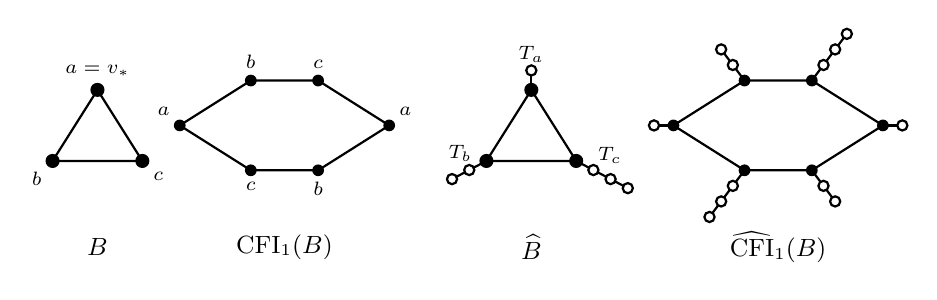
\begin{tikzpicture}[
  scale=.95,
  base/.style={circle,fill,inner sep=1.8pt},
  cfi/.style={circle,fill,inner sep=1.5pt},
  att/.style={circle,draw,fill=white,inner sep=1.3pt},
  lab/.style={font=\scriptsize,inner sep=1.5pt},
  line width=.8pt,
  every node/.style={font=\small},
]
\def\treeA#1#2{\draw (#1)--++(#2:.26) node[att]{};}
\def\treeB#1#2{\draw (#1)--++(#2:.26) node[att]{}--++(#2:.26) node[att]{};}
\def\treeC#1#2{\draw (#1)--++(#2:.26) node[att]{}--++(#2:.26) node[att]{}
                --++(#2:.26) node[att]{};}
\pgfmathsetmacro{\baseAngle}{atan2(.95/3,.6)}
\pgfmathsetmacro{\cfiAngle}{atan2(.6,.45)}
\foreach \attached in {0,1} {
  \begin{scope}[xshift={5.8*\attached cm}]
    \coordinate (a) at (0,.55);
    \coordinate (b) at (-.6,-.4);
    \coordinate (c) at (.6,-.4);
    \draw (a)--(b)--(c)--cycle;
    \ifnum\attached=0
      \node[base,label={[lab]above:$a=v_*$}] at (a) {};
      \node[base,label={[lab]below left:$b$}] at (b) {};
      \node[base,label={[lab]below right:$c$}] at (c) {};
      \node at (0,-1.55) {$B$};
    \else
      \treeA{a}{90}
      \treeB{b}{180+\baseAngle}
      \treeC{c}{360-\baseAngle}
      \node[lab,above] at (0,.85) {$T_a$};
      \node[lab,above] at (-.95,-.48) {$T_b$};
      \node[lab,above] at (1.05,-.5) {$T_c$};
      \foreach \v in {a,b,c} \node[base] at (\v) {};
      \node at (0,-1.55) {$\widehat B$};
    \fi
    \begin{scope}[xshift={(2.5+.8*\attached)*1cm}]
      \coordinate (a0) at (-1.4,.075);
      \coordinate (b0) at (-.45,.675);
      \coordinate (c0) at (.45,.675);
      \coordinate (a1) at (1.4,.075);
      \coordinate (b1) at (.45,-.525);
      \coordinate (c1) at (-.45,-.525);
      \draw (a0)--(b0)--(c0)--(a1)--(b1)--(c1)--cycle;
      \ifnum\attached=0
        \node[cfi,label={[lab]above left:$a$}] at (a0) {};
        \node[cfi,label={[lab]above:$b$}] at (b0) {};
        \node[cfi,label={[lab]above:$c$}] at (c0) {};
        \node[cfi,label={[lab]above right:$a$}] at (a1) {};
        \node[cfi,label={[lab]below:$b$}] at (b1) {};
        \node[cfi,label={[lab]below:$c$}] at (c1) {};
        \node at (0,-1.55) {$\CFI_1(B)$};
      \else
        \treeA{a0}{180} \treeA{a1}{0}
        \treeB{b0}{180-\cfiAngle} \treeB{b1}{360-\cfiAngle}
        \treeC{c0}{\cfiAngle}     \treeC{c1}{180+\cfiAngle}
        \foreach \v in {a0,b0,c0,a1,b1,c1} \node[cfi] at (\v) {};
        \node at (0,-1.55) {$\widehat{\CFI}_1(B)$};
      \fi
    \end{scope}
  \end{scope}
}
\end{tikzpicture}
\caption{A CFI-compatible rooted product for $B=K_3$ with $v_*=a$.
The hexagon labels indicate the base vertices of the fibres.
The attached paths $T_a,T_b,T_c$ have lengths one, two and three;
each vertex in the fibre over $z$ receives a copy of $T_z$.}
\label{fig:ss-cfi-example}
\end{figure}


\begin{lemma}\label{lem:ss-attachments}
Let $\mathcal C$ be a minor-closed graph class and $B$ a connected graph
such that $\CFI_0(B)\equiv_{\mathcal C}\CFI_1(B)$.
For any family of rooted graphs $(T_z)_{z\in V(B)}$, the CFI-compatible
rooted products satisfy
$\widehat{\CFI}_0(B)\equiv_{\mathcal C}\widehat{\CFI}_1(B)$.
\end{lemma}
\begin{proof}
Fix $F\in\mathcal C$.
We prove that, for $i\in\{0,1\}$,
\begin{equation}\label{eq:ss-attachment-count}
 \hom(F,\widehat{\CFI}_i(B))=
 \sum_{\eta:F\to\widehat B}\hom_{\chi_\eta}(Q_\eta,\CFI_i(B)),
\end{equation}
where, for each homomorphism $\eta:F\to\widehat B$, the graph $Q_\eta$
and the homomorphism $\chi_\eta:Q_\eta\to B$ are defined below.
The graph $Q_\eta$ is obtained from $F$ by contracting the connected
components of a subgraph of $F$ and replacing parallel edges by single edges, so
$Q_\eta$ is a minor of $F$, hence $Q_\eta\in\mathcal C$ because
$\mathcal C$ is minor-closed.
Since $\CFI_0(B)\equiv_{\mathcal C}\CFI_1(B)$ and $Q_\eta\in\mathcal C$,
we have $\hom(Q_\eta,\CFI_0(B))=\hom(Q_\eta,\CFI_1(B))$.
By \cref{eq:ss-lift-equality},
$\hom_{\chi_\eta}(Q_\eta,\CFI_0(B))=\hom_{\chi_\eta}(Q_\eta,\CFI_1(B))$.
Assuming \cref{eq:ss-attachment-count}, summing these equalities over $\eta$
gives $\hom(F,\widehat{\CFI}_0(B))=\hom(F,\widehat{\CFI}_1(B))$, which
proves the lemma.
It remains to define $Q_\eta$ and $\chi_\eta$ and to prove
\cref{eq:ss-attachment-count}.

For each homomorphism $\eta:F\to\widehat B$, define the following graphs and map.
Define a subgraph $F_\eta$ of $F$
with vertex set $V(F)$ by retaining an edge $vw\in E(F)$ if and only if
$\eta$ maps $vw$ to an edge of one of the attached copies $T_z$ in $\widehat B$.
Let $Q_\eta$ be the simple graph obtained from $F$ by contracting each
connected component of $F_\eta$ to one vertex and replacing parallel
edges by single edges; its vertices are the connected components of $F_\eta$.
Two distinct components are adjacent in $Q_\eta$ if and only if an edge of
$F$ has one endpoint in each component.
Every vertex of $\widehat B$ lies in exactly one attached copy, and the
edges of $F_\eta$ map into attached copies, so for each connected
component $K$ of $F_\eta$ there is a unique $z\in V(B)$ whose copy of
$T_z$ contains $\eta(K)$; we define $\chi_\eta(K)=z$.
If $vw\in E(F)$ has $v\in K$ and $w\in L$ for distinct components $K,L$, then
$\eta(v)\eta(w)$ is an edge of $B$ with endpoints $\chi_\eta(K)$ and
$\chi_\eta(L)$.
Hence $\chi_\eta:Q_\eta\to B$ is a homomorphism.

To prove \cref{eq:ss-attachment-count}, we fix $\eta$ and construct a
bijection between homomorphisms
$f:F\to\widehat{\CFI}_i(B)$ satisfying $\widehat\pi_i\circ f=\eta$
and lifts $h:Q_\eta\to\CFI_i(B)$ of $\chi_\eta$.
Given such an $f$, each connected component $K$ of $F_\eta$ maps
into a single attached copy, since every edge of $K$ projects into some
$T_z$. Let $h(K)$ be the root of this copy.
Then $\pi_i\circ h=\chi_\eta$, and edges between components map to edges
of $\CFI_i(B)$, so $h$ is a lift of $\chi_\eta$.

Conversely, let $h$ be a lift of $\chi_\eta$.
For each component $K$ of $F_\eta$, a copy of $T_{\chi_\eta(K)}$
is attached at $h(K)$ because $\pi_i(h(K))=\chi_\eta(K)$.
The projection $\widehat\pi_i$ maps this copy isomorphically onto
the copy of $T_{\chi_\eta(K)}$ in $\widehat B$.
For each $v\in K$, there is therefore a unique vertex $f(v)$ in the
copy rooted at $h(K)$ such that $\widehat\pi_i(f(v))=\eta(v)$.
Edges within a component are preserved by this isomorphism.
If $vw\in E(F)$ has $v\in K$ and $w\in L$ for distinct components $K,L$, then $\eta(v)$ and
$\eta(w)$ are roots. Hence $f(v)=h(K)$ and $f(w)=h(L)$, which are
adjacent because $h$ is a homomorphism.
The map $f\mapsto h$ and the map $h\mapsto f$ are inverse to each
other, which proves the bijection.
Summing over $\eta:F\to\widehat B$ proves \cref{eq:ss-attachment-count}.
\end{proof}

We next choose the attached graphs to obtain simple spectrum
(\cref{lem:ss-cfi-spectrum}).
A \emph{rooted subcubic caterpillar} is a tree obtained from a nonempty path
by attaching at most one new leaf to each path vertex and choosing an
endpoint of the path as the root. This path is called its \emph{spine}.
Thus the maximum degree is at most three and
the root degree is at most two; these bounds are used for the degree
bound in \cref{lem:ss-cfi-spectrum}.
The family $\mathcal T$ consists of the rooted subcubic caterpillars
obtained from $K_2$ rooted at an endpoint by zero or more applications
of the following two operations.
For a tree with root $r$, operation $X$ adds two new vertices $r',v$
and the edges $r'v,vr$, making $r'$ the new root.
Operation $Y$ adds a new root $r'$ and a new leaf $v$, with edges
$rr',r'v$ (\cref{fig:ss-operations}).

\begin{figure}[tb]
\centering
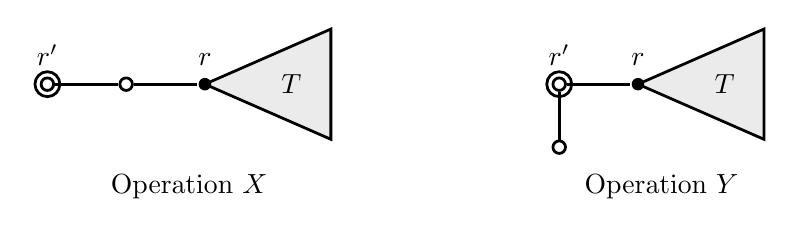
\begin{tikzpicture}[
  line width=1pt,
  old/.style={circle,fill,inner sep=1.6pt},
  new/.style={circle,draw,fill=white,inner sep=1.6pt},
  tree/.style={draw,fill=black!8},
]
\begin{scope}
  \draw[tree] (0,0) -- (1.6,0.7) -- (1.6,-0.7) -- cycle;
  \node at (1.1,0) {$T$};
  \node[old,label=above:$r$] (r) at (0,0) {};
  \node[new] (u) at (-1,0) {};
  \node[new,label=above:$r'$] (s) at (-2,0) {};
  \draw (s) -- (u) -- (r);
  \draw (s) circle (4.5pt);
  \node at (-0.2,-1.3) {Operation $X$};
\end{scope}
\begin{scope}[xshift=5.5cm]
  \draw[tree] (0,0) -- (1.6,0.7) -- (1.6,-0.7) -- cycle;
  \node at (1.1,0) {$T$};
  \node[old,label=above:$r$] (r) at (0,0) {};
  \node[new,label=above:$r'$] (s) at (-1,0) {};
  \node[new] (l) at (-1,-0.8) {};
  \draw (l) -- (s) -- (r);
  \draw (s) circle (4.5pt);
  \node at (0.3,-1.3) {Operation $Y$};
\end{scope}
\end{tikzpicture}
\caption{The operations $X$ and $Y$ applied to a rooted subcubic
caterpillar $T$ with root $r$. New vertices are white, and the new
root $r'$ is circled.}
\label{fig:ss-operations}
\end{figure}

We compute the characteristic polynomial of each $T\in\mathcal T$
recursively along its construction.
The adjacency matrix of a graph $H$ is denoted by $A_H$.
For the root $r$ of $T$, let $p_T(\lambda)=\det(\lambda I-A_T)$ and
$q_T(\lambda)=\det(\lambda I-A_{T-r})$ be the characteristic polynomials of $T$ and
$T-r$, respectively.
For a nonzero column $\xi=(p,q)^{\top}\in\R^2$, let
$[\xi]=[p:q]\in\mathbb P^1(\R)$ denote its span, identified with $p/q$ when $q\ne0$
and with $\infty$ when $q=0$.
In \cref{lem:ss-separation}, the eigenvalue multiplicities of the
rooted products depend on each attached tree $T$ only through the point
$h_T(\lambda)=[p_T(\lambda):q_T(\lambda)]$
(see \cref{lem:ss-rooted-multiplicity}).
We show that this point is defined for every real $\lambda$, that is,
$p_T(\lambda)$ and $q_T(\lambda)$ never vanish together.
The starting pair for rooted $K_2$ is
$(p_{K_2}(\lambda),q_{K_2}(\lambda))=(\lambda^2-1,\lambda)$.
By cofactor expansion, the operations $X$ and $Y$
transform the column $(p_T(\lambda),q_T(\lambda))^{\top}$ by multiplication
with the respective matrices
\begin{equation}\label{eq:ss-recurrence}
 \begin{aligned}
 \mathbf{X}_\lambda&=\begin{pmatrix}\lambda^2-1&-\lambda\\\lambda&-1\end{pmatrix},
 &\mathbf{Y}_\lambda&=\begin{pmatrix}\lambda^2-1&-\lambda\\\lambda&0\end{pmatrix}.
 \end{aligned}
\end{equation}
At $\lambda=0$, the recurrence \cref{eq:ss-recurrence} gives
$p_T(0)=(-1)^{|V(T)|/2}$ and $q_T(0)=0$.
These values are used for nonsingularity in \cref{lem:ss-separation}.
At $\lambda\ne0$, the starting pair is nonzero and both
matrices in \cref{eq:ss-recurrence} are invertible, so they carry
nonzero pairs to nonzero pairs.
Thus $h_T(\lambda)$ is defined for every real $\lambda$.

\begin{lemma}\label{lem:ss-caterpillars}
For any finite list of pairs
$(\lambda_j,a_j)\in\R^\times\times\mathbb P^1(\R)$, there is a tree
$T\in\mathcal T$ with $h_T(\lambda_j)\ne a_j$
for every $j$.
\end{lemma}
\begin{proof}
Let $\omega$ be a finite composition of the construction operations
$X,Y$, and let $T=\omega(K_2)$.
For each $j$, let $M_{\omega,j}$ be the matrix product obtained by
replacing each $X$ by $\mathbf{X}_{\lambda_j}$, each $Y$ by
$\mathbf{Y}_{\lambda_j}$, and composition by matrix multiplication.
For the empty composition, $M_{\omega,j}=I$.
Let $\nu_j=(p_{K_2}(\lambda_j),q_{K_2}(\lambda_j))^{\top}
=(\lambda_j^2-1,\lambda_j)^{\top}$.
Then $(p_T(\lambda_j),q_T(\lambda_j))^{\top}=M_{\omega,j}\nu_j$
by \cref{eq:ss-recurrence}.
Therefore, it suffices to find a composition $\omega$ such that
$[M_{\omega,j}\nu_j]\ne a_j$ for every $j$.

We express the conditions $[M_{\omega,j}\nu_j]\ne a_j$ for all $j$
as the nonvanishing of a linear functional on a tensor product.
For each $j$, define the linear functional
$\ell_j:\R^2\to\R$ by
\begin{equation}\label{eq:ss-avoidance-factors}
 \ell_j(p,q)=
 \begin{cases}
  p-a_jq,&a_j\in\R,\\
  q,&a_j=\infty.
 \end{cases}
\end{equation}
Let
$\nu=\bigotimes_j\nu_j$, $\ell=\bigotimes_j\ell_j$,
$\mathbf{X}=\bigotimes_j\mathbf{X}_{\lambda_j}$ and
$\mathbf{Y}=\bigotimes_j\mathbf{Y}_{\lambda_j}$,
where $\otimes$ is the tensor product.
Define $M_\omega$ in the same way using $\mathbf{X},\mathbf{Y}$.
Multiplication of tensor products gives
$M_\omega=\bigotimes_jM_{\omega,j}$.
Since $\ell$ is a tensor product of functionals,
\begin{equation}\label{eq:ss-positive-word}
 \ell(M_\omega\nu)=\prod_j\ell_j(M_{\omega,j}\nu_j),
\end{equation}
and each factor is nonzero exactly when
$h_T(\lambda_j)\ne a_j$.
Thus the avoidance conditions hold exactly when $\ell(M_\omega\nu)\ne0$.

It suffices to find a finite product $W$ of the matrices
$\mathbf{X}^{\pm1},\mathbf{Y}^{\pm1}$ with $\ell(W\nu)\ne0$.
Since every $\lambda_j\ne0$, the matrices $\mathbf{X},\mathbf{Y}$ are
invertible. By the Cayley--Hamilton theorem, their inverses are
polynomials in $\mathbf{X},\mathbf{Y}$, respectively.
Substituting these polynomial expressions into $W$ and expanding gives
a finite sum $W=\sum_i c_iM_{\omega_i}$, where $c_i\in\R$ and each
$\omega_i$ is a composition of the construction operations $X,Y$.
Consequently, $\ell(W\nu)=\sum_i c_i\ell(M_{\omega_i}\nu)\ne0$
implies $\ell(M_{\omega_i}\nu)\ne0$ for some $i$.
By \cref{eq:ss-positive-word}, the tree $T=\omega_i(K_2)$ then satisfies
$h_T(\lambda_j)\ne a_j$ for every $j$.

We now construct such a product $W$.
For $\lambda\ne0$, the matrices in \cref{eq:ss-recurrence} act on
$\mathbb P^1(\R)$ by multiplication of column representatives.
Let $D_\lambda=\mathbf{X}_\lambda^{-1}\mathbf{Y}_\lambda$.
On $\mathbb P^1(\R)$, $D_\lambda$ acts by
$t\mapsto\lambda^{-2}t+\lambda^{-1}$.
The starting value is $h_{K_2}(\lambda)=\lambda-\lambda^{-1}=\mathbf{Y}_\lambda\infty$.
Since $\mathbf{Y}_\lambda^{-1}\infty=0$, we have
$\mathbf{Y}_\lambda^{-2}h_{K_2}(\lambda)=0$.
Thus $D_\lambda^m\mathbf{Y}_\lambda^{-2}$ sends the starting value to
$\lambda^{-1}\sum_{k=0}^{m-1}\lambda^{-2k}$.
These values are strictly monotone in $m$ for every real $\lambda\ne0$,
so each $a_j$ is attained for at most one $m$ at $\lambda=\lambda_j$.
Choose a positive integer $m$ such that
$[D_{\lambda_j}^m\mathbf{Y}_{\lambda_j}^{-2}\nu_j]\ne a_j$ for every $j$.
Then $W=(\mathbf{X}^{-1}\mathbf{Y})^m\mathbf{Y}^{-2}$ satisfies
$\ell(W\nu)=\prod_j\ell_j(D_{\lambda_j}^m\mathbf{Y}_{\lambda_j}^{-2}\nu_j)\ne0$,
as required.
\end{proof}

For a base graph with edge weights, the rooted product retains the
original edge weights, and the edges of each $T_z$ have weight one.

\begin{lemma}\label{lem:ss-rooted-multiplicity}
Let $B$ be a graph with real edge weights.
For each $z\in V(B)$, let $T_z\in\mathcal T$, and let $\widehat B$ be the
rooted product of $B$ with $(T_z)_{z\in V(B)}$.
For $\lambda\in\R$, define
\begin{equation}\label{eq:ss-rooted-core}
 K^\lambda=\diag(p_{T_z}(\lambda))_{z\in V(B)}
       -A_B\diag(q_{T_z}(\lambda))_{z\in V(B)}.
\end{equation}
Then
\begin{equation}\label{eq:ss-multiplicity}
 \dim\ker(\lambda I-A_{\widehat B})=\dim\ker K^\lambda.
\end{equation}
\end{lemma}
\begin{proof}
Fix $\lambda\in\R$ and put
$p_z=p_{T_z}(\lambda)$ and $q_z=q_{T_z}(\lambda)$.
Let $J=\{z\in V(B):q_z\ne0\}$ and $J^c=V(B)\setminus J$, and define
\begin{equation}\label{eq:ss-schur-core}
 \Sigma=\diag(p_z/q_z)_{z\in J}-A_{B}[J,J],
\end{equation}
where $A_{B}[J,J]$ is the principal submatrix indexed by $J$.
We will show that both sides of \cref{eq:ss-multiplicity} equal
$\dim\ker \Sigma$.
When $J=\varnothing$, we have $\dim\ker \Sigma=0$.

We first consider $K^\lambda$.
For $z\in J^c$, we have $q_z=0$ and $p_z\ne0$, so column $z$
has the single nonzero entry $p_z$ in row $z$.
Ordering $J$ before $J^c$ therefore gives
\begin{equation}\label{eq:ss-core-partition}
 K^\lambda=
 \begin{pmatrix}
 K^\lambda[J,J]&0\\
 K^\lambda[J^c,J]&\diag(p_z)_{z\in J^c}
 \end{pmatrix}.
\end{equation}
Since the lower-right block is invertible,
$\dim\ker K^\lambda=\dim\ker K^\lambda[J,J]$.
Also $K^\lambda[J,J]=\Sigma\diag(q_z)_{z\in J}$ with every $q_z\ne0$,
so $\dim\ker K^\lambda=\dim\ker \Sigma$.

It remains to prove $\dim\ker(\lambda I-A_{\widehat B})=\dim\ker \Sigma$.
Let $\widehat{B[J]}$ be the rooted product of the induced base graph
$B[J]$ with $(T_z)_{z\in J}$.
We first prove the deletion identity
\begin{equation}\label{eq:ss-tree-deletion}
 \dim\ker(\lambda I-A_{\widehat B})
 =\dim\ker(\lambda I-A_{\widehat{B[J]}}).
\end{equation}
To prove \cref{eq:ss-tree-deletion}, we delete from $\widehat B$
the whole copies $T_z$ with $z\in J^c$, including their roots, one at a time.
At each step, let $L$ be the remaining induced subgraph of $\widehat B$.
For the copy $T_z$ to be removed, put $D_z=\lambda I-A_{T_z}$ and
$R_z=\lambda I-A_{L-V(T_z)}$.
Let $e_z$ be the root coordinate vector in $\R^{V(T_z)}$, and let
$b_z$ be the vector of edge weights from the root to $V(L)\setminus V(T_z)$.
Ordering $V(T_z)$ first gives
\begin{equation}\label{eq:ss-whole-tree-block}
 \lambda I-A_L=
 \begin{pmatrix}D_z&-e_zb_z^{\top}\\-b_ze_z^{\top}&R_z\end{pmatrix}.
\end{equation}
Here $D_z$ is invertible because $\det D_z=p_z\ne0$.
Cramer's rule gives $e_z^{\top}D_z^{-1}e_z=q_z/p_z=0$.
Thus the Schur complement of $D_z$ in \cref{eq:ss-whole-tree-block} is
\begin{equation}\label{eq:ss-zero-tree-correction}
 R_z-b_z(e_z^{\top}D_z^{-1}e_z)b_z^{\top}
 =R_z-\frac{q_z}{p_z}b_zb_z^{\top}=R_z.
\end{equation}
Since $D_z$ is invertible,
$\dim\ker(\lambda I-A_L)=\dim\ker R_z$.
The remaining matrix is exactly $R_z=\lambda I-A_{L-V(T_z)}$,
so the same calculation applies after each deletion.
Deleting all copies indexed by $J^c$ therefore proves
\cref{eq:ss-tree-deletion}.

It remains to show that
$\dim\ker(\lambda I-A_{\widehat{B[J]}})=\dim\ker \Sigma$.
For $z\in J$, put $E_z=\lambda I-A_{T_z-r_z}$, and let
$c_z$ be the vector of edge weights from $r_z$ to the non-root vertices
of $T_z$.
Let $E=\bigoplus_{z\in J}E_z$, and let $C$ have rows indexed by these
non-root vertices and columns indexed by $J$.
Column $z$ of $C$ equals $c_z$ on $V(T_z)\setminus\{r_z\}$ and is
zero elsewhere.
Ordering all non-root vertices before the roots gives
\begin{equation}\label{eq:ss-nonroot-block}
 \lambda I-A_{\widehat{B[J]}}=
 \begin{pmatrix}E&-C\\-C^{\top}&\lambda I-A_{B}[J,J]\end{pmatrix}.
\end{equation}
Every $E_z$ is invertible because $\det E_z=q_z\ne0$.
The determinant formula for the Schur complement of $E_z$ in
$\lambda I-A_{T_z}$ gives
$p_z=q_z(\lambda-c_z^{\top}E_z^{-1}c_z)$.
Since distinct columns of $C$ are supported on distinct blocks of $E$,
the Schur complement of $E$ in \cref{eq:ss-nonroot-block} is
\begin{equation}\label{eq:ss-root-schur}
 \lambda I-A_{B}[J,J]-C^{\top}E^{-1}C
 =\diag(p_z/q_z)_{z\in J}-A_{B}[J,J]=\Sigma.
\end{equation}
Since $E$ is invertible, \cref{eq:ss-tree-deletion,eq:ss-root-schur} give
\begin{equation}\label{eq:ss-kernel-reduction}
 \dim\ker(\lambda I-A_{\widehat B})
 =\dim\ker \Sigma
 =\dim\ker K^\lambda,
\end{equation}
which proves \cref{eq:ss-multiplicity}.
For unweighted rooted products, the determinant identity
$\det(\lambda I-A_{\widehat B})=\det K^\lambda$
is \cite[Theorem~2.1]{GodsilMcKay1978}.
\end{proof}

\begin{lemma}\label{lem:ss-separation}
Let $Z$ be a finite set, and let $B_1,\ldots,B_s$ be connected graphs
with nonzero real edge weights and pairwise distinct nonempty vertex sets
$Z_i=V(B_i)\subseteq Z$.
There is a family $(T_z)_{z\in Z}$ of trees in $\mathcal T$ such that the rooted products
of $B_i$ with $(T_z)_{z\in Z_i}$ are nonsingular and have simple, pairwise
disjoint spectra.
\end{lemma}
\begin{proof}
Put $d=|Z|$, and let $A_{B_i}$ be the weighted adjacency matrix of $B_i$.
For $\alpha,\beta\in\mathbb C^Z$, let
\begin{equation}\label{eq:ss-core}
 K_i(\alpha,\beta)=\diag(\alpha_z)_{z\in Z_i}-A_{B_i}\diag(\beta_z)_{z\in Z_i}.
\end{equation}
For a projective point $a=([\alpha_z:\beta_z])_{z\in Z}$,
rescaling each homogeneous representative multiplies $K_i(\alpha,\beta)$
on the right by an invertible diagonal matrix.
Thus $\dim\ker K_i(\alpha,\beta)$ depends only on $a$.
Fix trees $T_z\in\mathcal T$, and write $\widehat B_i$ for the rooted
product of $B_i$ with $(T_z)_{z\in Z_i}$.
For $\lambda\in\R$, let
$K_i^\lambda=K_i((p_{T_z}(\lambda))_{z\in Z},(q_{T_z}(\lambda))_{z\in Z})$.

We define closed subsets $\mathcal V_i^{(k)}$ for $k\in\{1,2\}$
and $\mathcal E$ of $(\mathbb P^1(\mathbb C))^Z$ by
\begin{equation}\label{eq:ss-bad-sets}
 \begin{aligned}
 \mathcal V_i^{(k)}&=\{([\alpha_z:\beta_z])_{z\in Z}:\dim\ker K_i(\alpha,\beta)\ge k\}, &
 \mathcal E&=\bigcup_i\mathcal V_i^{(2)}
       \cup\bigcup_{i\ne i'}(\mathcal V_i^{(1)}\cap \mathcal V_{i'}^{(1)}).
 \end{aligned}
\end{equation}
These conditions are independent of the homogeneous representatives.
By \cref{lem:ss-rooted-multiplicity}, for $\lambda\in\R$ and
$a=(h_{T_z}(\lambda))_{z\in Z}$, the number $\lambda$ is an eigenvalue
of $\widehat B_i$ of multiplicity at least $k$ exactly when
$a\in\mathcal V_i^{(k)}$.
It is an eigenvalue of both $\widehat B_i$ and $\widehat B_{i'}$ exactly
when $a\in\mathcal V_i^{(1)}\cap\mathcal V_{i'}^{(1)}$.
At $\lambda=0$, the matrix $K_i^0$ is invertible
because $q_{T_z}(0)=0$ and $p_{T_z}(0)\ne0$.
Thus the products $\widehat B_i$ are nonsingular.
Their spectra are simple and pairwise disjoint exactly when
\begin{equation}\label{eq:ss-bad}
 (h_{T_z}(\lambda))_{z\in Z}\notin\mathcal E
 \quad\text{for every }\lambda\in\R^\times.
\end{equation}

We next prove $\dim\mathcal E\le d-2$ over $\mathbb C$.
The polynomial $\det(\diag(t)-A_{B_i})$ in the variables $(t_z)_{z\in Z_i}$
is irreducible because $B_i$ is connected
\cite[Lemma~4.1]{AlAhmadieh2026}.
Substituting $t_z=\alpha_z/\beta_z$ and clearing denominators gives the
determinant of the matrix in \cref{eq:ss-core}, as a polynomial in the
homogeneous representatives $(\alpha_z,\beta_z)$.
Its projective zero set is $\mathcal V_i^{(1)}$, so
$\mathcal V_i^{(1)}$ is an irreducible hypersurface.
For each $z\in Z$, let $a^{(z)}\in(\mathbb P^1(\mathbb C))^Z$ have
coordinate $[0:1]$ at $z$ and $[1:0]$ elsewhere.
Using these homogeneous coordinates, $\dim\ker K_i(\alpha,\beta)$ is one
if $z\in Z_i$ and zero otherwise.
For $i\ne i'$, choose $z$ in the symmetric difference of $Z_i$ and
$Z_{i'}$; then $a^{(z)}$ lies in exactly one of $\mathcal V_i^{(1)}$ and
$\mathcal V_{i'}^{(1)}$.
Thus the $\mathcal V_i^{(1)}$ are distinct, so each intersection
$\mathcal V_i^{(1)}\cap \mathcal V_{i'}^{(1)}$ has dimension at most $d-2$.
For each $i$ and each $z\in Z_i$, the point $a^{(z)}$ lies in
$\mathcal V_i^{(1)}\setminus\mathcal V_i^{(2)}$.
Thus $\mathcal V_i^{(2)}$ is a proper closed subset of
$\mathcal V_i^{(1)}$ and also has dimension at most $d-2$.
The union defining $\mathcal E$ therefore has dimension at most $d-2$.

Since $\mathbb C^\times\times\mathcal E$ has dimension at most $d-1$,
we can choose $d$ trees to satisfy \cref{eq:ss-bad} as follows.
We enumerate $Z$ as $\{1,\ldots,d\}$.
For fixed trees $T_1,\ldots,T_j$, let $P_j$ be the set of pairs
$(\lambda,a)$ with $\lambda\in\R^\times$,
$a\in\mathcal E\cap(\mathbb P^1(\R))^Z$, and
$a_z=h_{T_z}(\lambda)$ for all $z\le j$.
Let $\Omega_j$ be the Zariski closure of $P_j$ in
$\mathbb C^\times\times\mathcal E$.
Then $\dim\Omega_0\le d-1$.
We choose $T_{j+1}$ so that $\Omega_{j+1}$ contains no irreducible
component of $\Omega_j$.
By definition, $P_{j+1}\subseteq P_j$, so $\Omega_{j+1}\subseteq\Omega_j$.
Every pair $(\lambda,a)\in P_{j+1}$ satisfies
$a_{j+1}=h_{T_{j+1}}(\lambda)$. In homogeneous coordinates this is
equivalent to
\begin{equation}\label{eq:ss-cut}
 \alpha_{j+1}q_{T_{j+1}}(\lambda)-\beta_{j+1}p_{T_{j+1}}(\lambda)=0.
\end{equation}
This polynomial equation also holds on the Zariski closure
$\Omega_{j+1}$.
It therefore suffices to choose $T_{j+1}$ so that \cref{eq:ss-cut}
fails at one point of every irreducible component of $\Omega_j$.

For each irreducible component $\mathcal W$ of $\Omega_j$, we choose a pair
$(\lambda_{\mathcal W},a_{\mathcal W})\in P_j\cap\mathcal W$ that lies in no other irreducible component
of $\Omega_j$.
Such a pair exists, because otherwise $P_j$ would lie in the closed
union of the other components, contradicting the definition of
$\Omega_j$ as the Zariski closure of $P_j$.
The pairs $(\lambda_{\mathcal W},(a_{\mathcal W})_{j+1})$, one for each irreducible component
$\mathcal W$ of $\Omega_j$, form a finite list in
$\R^\times\times\mathbb P^1(\R)$.
By \cref{lem:ss-caterpillars} there is therefore a tree
$T_{j+1}\in\mathcal T$ with
$h_{T_{j+1}}(\lambda_{\mathcal W})\ne(a_{\mathcal W})_{j+1}$ for every $\mathcal W$.
Thus \cref{eq:ss-cut} fails at $(\lambda_{\mathcal W},a_{\mathcal W})$ in every irreducible
component $\mathcal W$ of $\Omega_j$.
Thus $\Omega_{j+1}$ contains no irreducible component of $\Omega_j$,
so $\dim\Omega_{j+1}<\dim\Omega_j$.
If $\Omega_j$ is empty, we choose the remaining trees arbitrarily.
Since $\dim\Omega_0\le d-1$ and the dimension strictly decreases
whenever $\Omega_j$ is nonempty, $\Omega_d=\varnothing$, so $P_d=\varnothing$.
Hence \cref{eq:ss-bad} holds, and the lemma follows.
\end{proof}

\begin{lemma}\label{lem:ss-cfi-blocks}
Let $\Gamma$ be a connected cubic graph, and let $S$ be its subdivision
with one new vertex on each edge.
Choose the distinguished vertex $v_*$ of $\CFI_1(S)$ in $V(\Gamma)$.
Fix trees $(T_z)_{z\in V(S)}$ in $\mathcal T$ and form the
CFI-compatible rooted products $\widehat{\CFI}_i(S)$ for $i\in\{0,1\}$.
The subdivision has vertex set $V(S)=V(\Gamma)\sqcup E(\Gamma)$,
where the new vertex on the edge $e$ is denoted by $e$.
Let $S_0$ be $S$ with every edge weighted $\sqrt2$, and for
$e=vw\in E(\Gamma)$ let $S_e$ be the path with edges $ve,ew$ and the
same edge weights.
Write $\widehat S_0$ and $\widehat S_e$ for their rooted products with
the corresponding trees $T_z$.
For each $i\in\{0,1\}$, the adjacency matrix of $\widehat{\CFI}_i(S)$
is orthogonally similar to
\begin{equation}\label{eq:ss-rooted-blocks}
 A_{\widehat S_0}\oplus\bigoplus_{e\in E(\Gamma)}A_{\widehat S_e}.
\end{equation}

\end{lemma}
\begin{proof}
We prove the decomposition by specifying the corresponding subspaces
and orthonormal bases.
Fix $i\in\{0,1\}$.
For $v\in V(\Gamma)$, the fibre over $v$ is indexed by $\Xi_i(v)$, which
consists of the four vectors in $\mathbb F_2^{E_S(v)}$ of the
prescribed parity.
For a subdivision vertex $e$, the fibre over $e$ is indexed by
$\Xi_i(e)=\{(0,0),(1,1)\}$; we write $b$ for $(b,b)$.
The vertices of $\widehat{\CFI}_i(S)$ are indexed by $(z,\xi,x)$, with $z\in V(S)$,
$\xi\in \Xi_i(z)$ and $x\in V(T_z)$.
The coordinate $(z,\xi,r_z)$ denotes the original CFI vertex $(z,\xi)$,
where $r_z$ is the root of $T_z$.

On $\Xi_i(v)$, we use the basis $\phi_{v,0}(\xi)=1/2$ and
$\phi_{v,e}(\xi)=(-1)^{\xi_e}/2$ for the three edges $e$ incident with $v$.
On $\Xi_i(e)$, we use the basis $\psi_{e,0}(b)=1/\sqrt2$ and
$\psi_{e,1}(b)=(-1)^b/\sqrt2$.
These bases are orthonormal under either parity constraint.
On $\Xi_i(v)$, any two incident coordinates range exactly once over
$\mathbb F_2^2$, because parity determines the third.
Thus $\sum_{\xi\in \Xi_i(v)}\phi_{v,e}(\xi)=0$,
$\langle\phi_{v,e},\phi_{v,e'}\rangle=0$ for distinct incident edges $e,e'$,
and $\lVert\phi_{v,e}\rVert=1$.
The functions $\psi_{e,0},\psi_{e,1}$ are orthonormal by the same two-point
calculation.

For $z\in V(S)$, $g\in\R^{\Xi_i(z)}$ and $x\in V(T_z)$,
let $g[x]\in\R^{V(\widehat{\CFI}_i(S))}$ be the function with value $g(\xi)$ at
$(z,\xi,x)$ for each $\xi\in \Xi_i(z)$ and zero elsewhere.
The functions $g[x]$ obtained from all basis vectors $g$ above and all
tree positions $x$ form an orthonormal basis of $\R^{V(\widehat{\CFI}_i(S))}$.
We define subspaces corresponding to $\widehat S_0$
and the graphs $\widehat S_e$.
Let $U_0$ be the subspace of functions constant in $\xi$ at each fixed $(z,x)$.
The subspace $U_0$ is spanned by $\phi_{v,0}[x]$ for $v\in V(\Gamma)$
and $x\in V(T_v)$, together with $\psi_{e,0}[x]$ for $e\in E(\Gamma)$
and $x\in V(T_e)$.
For each $e=vw$, let $U_e$ be spanned by $\phi_{v,e}[x]$, $\psi_{e,1}[x]$
and $\phi_{w,e}[x]$, with $x$ ranging over $V(T_v),V(T_e),V(T_w)$,
respectively.
These spanning sets partition the orthonormal basis.
For each subspace, we send each of its listed basis vectors $g[x]$ to the standard coordinate vector indexed
by $(z,x)$, where $g\in\R^{\Xi_i(z)}$.
This gives the isometric identifications
\begin{equation}\label{eq:ss-cfi-subspaces}
 \begin{aligned}
 U_0&\cong\R^{V(\widehat S_0)}, &
 U_e&\cong\R^{V(\widehat S_e)}\text{ for }e\in E(\Gamma).
 \end{aligned}
\end{equation}

We compute the adjacency matrix in this basis, starting with tree edges.
For $z\in V(S)$, write $(g_\kappa)_{\kappa=1}^{|\Xi_i(z)|}$ for its fibre basis.
Let $Q_z$ be the matrix whose $\kappa$th column is $g_\kappa$, so
$(Q_z)_{\xi\kappa}=g_\kappa(\xi)$ for $\xi\in \Xi_i(z)$.
The subgraph of $\widehat{\CFI}_i(S)$ induced by the vertices $(z,\xi,x)$ with
$\xi\in \Xi_i(z)$ and $x\in V(T_z)$ is the disjoint union of $|\Xi_i(z)|$ copies
of $T_z$. Its adjacency matrix in coordinates $(\xi,x)$ is $I\otimes A_{T_z}$,
because the same tree is attached at every vertex of the fibre.
The same basis change at every tree position is $Q_z\otimes I$, so
\begin{equation}\label{eq:ss-tree-blocks}
 (Q_z\otimes I)^{\top}(I\otimes A_{T_z})(Q_z\otimes I)
 =(Q_z^{\top}Q_z)\otimes A_{T_z}
 =I\otimes A_{T_z}.
\end{equation}
Thus the adjacency matrix of this induced subgraph has one block $A_{T_z}$
on each set $\{g_\kappa[x]:x\in V(T_z)\}$, with zero entries between these sets.
Each set lies in one of the subspaces $U_0,U_e$.

For an incidence $v\in e$, the root vertices
$(v,\xi,r_v)$ and $(e,b,r_e)$ are adjacent exactly when $\xi_e=b$.
Let $R_{v,e}$ be the matrix $R_{v,e}(\xi,b)=\delta_{\xi_e,b}$ of
this adjacency. It satisfies
\begin{equation}\label{eq:ss-fourier}
 \begin{aligned}
 R_{v,e}\psi_{e,0}&=\sqrt2\phi_{v,0}, &
 R_{v,e}\psi_{e,1}&=\sqrt2\phi_{v,e},
 \end{aligned}
\end{equation}
and, by orthonormality, $R_{v,e}^{\top}$ sends all other vectors
in the chosen basis of $\R^{\Xi_i(v)}$ to zero.
Thus the matrix of $R_{v,e}$ in these fibre bases has entry $\sqrt2$
at the row--column pairs $(\phi_{v,0},\psi_{e,0})$ and
$(\phi_{v,e},\psi_{e,1})$, and all other entries are zero.
Hence, in the stated bases of $U_0$ and $U_e$,
the submatrices indexed by root coordinates are $A_{S_0}$ and $A_{S_e}$,
respectively. \Cref{fig:ss-cfi-blocks} shows this decomposition for
$\Gamma=K_4$.
\begin{figure}[tb]
\centering
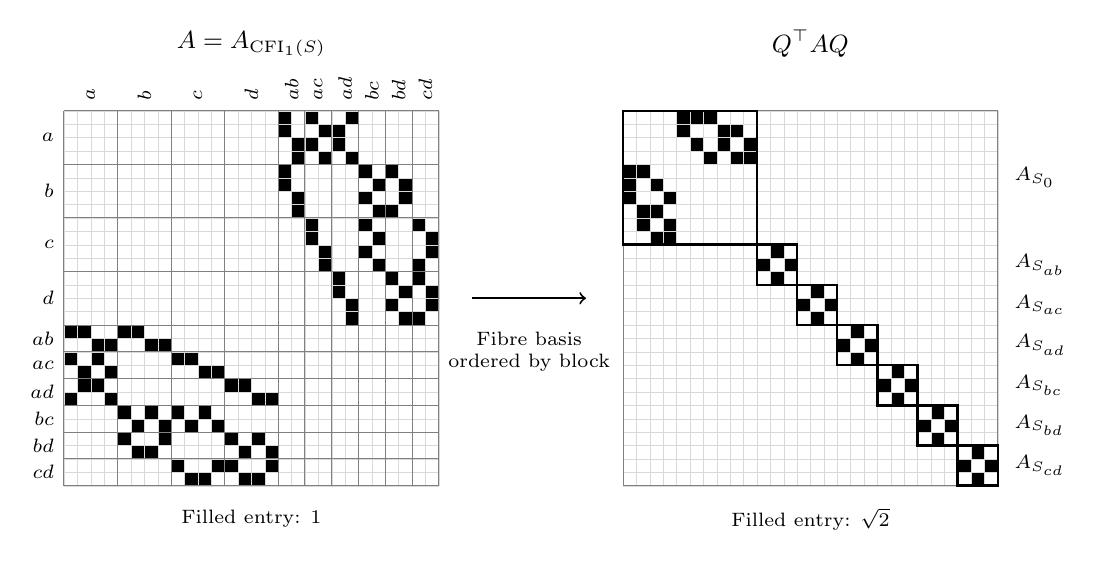
\begin{tikzpicture}[
  x=.17cm,y=-.17cm,
  entry/.style={fill=black},
  gridline/.style={draw=black!15,line width=.1pt},
  fibreline/.style={draw=black!50,line width=.35pt},
  block/.style={draw=black,line width=.9pt},
  every node/.style={font=\scriptsize,inner sep=1pt},
]
\node[font=\small] at (14,-5) {$A=A_{\CFI_1(S)}$};
\foreach \v/\e/\k in {
  0/0/0,0/1/1,0/2/2,
  1/0/0,1/3/1,1/4/2,
  2/1/0,2/3/1,2/5/2,
  3/2/0,3/4/1,3/5/2
} {
  \ifnum\v=0
    \def\fibrebits{0/0/0/1,1/0/1/0,2/1/0/0,3/1/1/1}
  \else
    \def\fibrebits{0/0/0/0,1/0/1/1,2/1/0/1,3/1/1/0}
  \fi
  \foreach \r/\first/\second/\third in \fibrebits {
    \ifcase\k\edef\bit{\first}\or\edef\bit{\second}\or\edef\bit{\third}\fi
    \pgfmathtruncatemacro{\row}{4*\v+\r}
    \pgfmathtruncatemacro{\col}{16+2*\e+\bit}
    \fill[entry] (\col,\row) rectangle ++(1,1);
    \fill[entry] (\row,\col) rectangle ++(1,1);
  }
}
\foreach \position in {0,...,28} {
  \draw[gridline] (\position,0)--(\position,28);
  \draw[gridline] (0,\position)--(28,\position);
}
\foreach \boundary in {0,4,8,12,16,18,20,22,24,26,28} {
  \draw[fibreline] (\boundary,0)--(\boundary,28);
  \draw[fibreline] (0,\boundary)--(28,\boundary);
}
\foreach \position/\name in {
  2/a,6/b,10/c,14/d,17/ab,19/ac,21/ad,23/bc,25/bd,27/cd
} {
  \node[anchor=west,rotate=90] at (\position,-.5) {$\name$};
  \node[anchor=east] at (-.5,\position) {$\name$};
}
\node at (14,30.5) {Filled entry: $1$};

\draw[->,line width=.7pt] (30.5,14)--(39,14);
\node[align=center] at (34.75,18) {Fibre basis\\ordered by block};

\begin{scope}[xshift=7.1cm]
  \node[font=\small] at (14,-5) {$Q^{\top}AQ$};
  \foreach \e/\u/\v in {0/0/1,1/0/2,2/0/3,3/1/2,4/1/3,5/2/3} {
    \pgfmathtruncatemacro{\subdivision}{4+\e}
    \foreach \endpoint in {\u,\v} {
      \fill[entry] (\subdivision,\endpoint) rectangle ++(1,1);
      \fill[entry] (\endpoint,\subdivision) rectangle ++(1,1);
    }
    \pgfmathtruncatemacro{\start}{10+3*\e}
    \foreach \r/\c in {0/1,1/0,1/2,2/1} {
      \fill[entry] ({\start+\c},{\start+\r}) rectangle ++(1,1);
    }
  }
  \foreach \position in {0,...,28} {
    \draw[gridline] (\position,0)--(\position,28);
    \draw[gridline] (0,\position)--(28,\position);
  }
  \draw[fibreline] (0,0) rectangle (28,28);
  \draw[block] (0,0) rectangle (10,10);
  \node[anchor=west] at (29,5) {$A_{S_0}$};
  \foreach \j/\e in {0/ab,1/ac,2/ad,3/bc,4/bd,5/cd} {
    \pgfmathtruncatemacro{\start}{10+3*\j}
    \draw[block] (\start,\start) rectangle ++(3,3);
    \node[anchor=west] at (29,{\start+1.5}) {$A_{S_{\e}}$};
  }
  \node at (14,30.5) {Filled entry: $\sqrt2$};
\end{scope}
\end{tikzpicture}
\caption{Block decomposition for the subdivision $S$ of $\Gamma=K_4$
on vertices $a,b,c,d$, with tree attachments omitted.
The left matrix groups the $28$ CFI vertices by fibre and uses odd parity
at $a$. Within fibres, the bit vectors are in lexicographic order,
with incident-edge coordinates ordered by their labels.
The columns of $Q$ are the fibre basis vectors from the proof, ordered
first by the ten constant directions and then by the three sign directions
over $v,e,w$ for each edge $e=vw$ of $K_4$.
The right matrix has one $10\times10$ block $A_{S_0}=\sqrt2 A_S$ and
six $3\times3$ blocks $A_{S_e}$; unfilled entries are zero.
Both CFI parities give the same right matrix.}
\label{fig:ss-cfi-blocks}
\end{figure}


Combining these root-coordinate matrices with the tree blocks in
\cref{eq:ss-tree-blocks} shows that the subspaces $U_0$ and $U_e$
are invariant and that the adjacency matrix of $\widehat{\CFI}_i(S)$ has the block diagonal form
\cref{eq:ss-rooted-blocks} in the stated bases.
\end{proof}

\begin{lemma}\label{lem:ss-cfi-spectrum}
Let $\Gamma$ be a connected cubic graph, and let $S$ be its subdivision
with one new vertex on each edge.
There is a family $(T_z)_{z\in V(S)}$ of trees in $\mathcal T$ such that the
CFI-compatible rooted products $\widehat{\CFI}_0(S)$ and $\widehat{\CFI}_1(S)$
are non-isomorphic, bipartite, cospectral, nonsingular graphs with
simple spectrum and maximum degree at most six.
\end{lemma}
\begin{proof}
Since the isomorphism type of $\CFI_1(S)$ is independent of the
distinguished vertex $v_*$, we choose $v_*\in V(\Gamma)$.
Let $S_0$ and $S_e$ be the weighted graphs from \cref{lem:ss-cfi-blocks}.
We apply \cref{lem:ss-separation} to these graphs,
with $Z=V(S)$.
They are connected and have nonzero edge weights. Their vertex sets
$V(S)$ and $\{v,e,w\}$ for $e=vw\in E(\Gamma)$ are pairwise distinct.
By that lemma, there is one tree $T_z\in\mathcal T$ for each
$z\in V(S)$ such that the rooted products $\widehat S_0$ and
$\widehat S_e$ are nonsingular and have simple, pairwise disjoint
spectra.
The block matrix in \cref{eq:ss-rooted-blocks} therefore has simple
spectrum and is nonsingular.
By \cref{lem:ss-cfi-blocks}, the adjacency matrices of
$\widehat{\CFI}_0(S)$ and $\widehat{\CFI}_1(S)$ are both
orthogonally similar to this matrix, so the two rooted products are
cospectral, nonsingular and have simple spectrum.

The graphs $\widehat{\CFI}_0(S)$ and $\widehat{\CFI}_1(S)$ are
non-isomorphic because their maximal subgraphs of minimum degree at least two
are the non-isomorphic graphs $\CFI_0(S)$ and $\CFI_1(S)$.
Both rooted products are bipartite, since each CFI graph is bipartite
and attaching trees preserves bipartiteness.
The CFI graphs have maximum degree four, and each attached tree is
subcubic with root degree at most two, so the rooted products have
maximum degree at most six.
\end{proof}

\begin{proof}[Proof of \cref{lem:ss-transfer}]
\Cref{lem:ss-cfi-spectrum} needs the subdivision of a connected cubic
graph as its base, so we first replace $B$ by such a base $S$ that
contains $B$ as a minor.
Let $t$ be an integer with $t\geq\max\{4,|V(B)|\}$, so that $B$ is a minor of $K_t$ and the
cycles below have length at least three.
Let $\Gamma$ be the connected cubic graph obtained from $K_t$ by
replacing each vertex with a cycle of length $t-1$ and attaching its
$t-1$ incident edges to distinct cycle vertices.
Let $S$ be the
subdivision of $\Gamma$ with one new vertex on each edge.
Contracting one edge at each subdivision vertex of $S$ gives $\Gamma$,
and contracting the replacement cycles of $\Gamma$ gives $K_t$, so $B$
is a minor of $S$.
Hence $\CFI_0(S)\equiv_{\mathcal C}\CFI_1(S)$ follows from the
assumption $\CFI_0(B)\equiv_{\mathcal C}\CFI_1(B)$ by
\cite[Corollary~5.7]{Roberson2026}.
Using the trees from \cref{lem:ss-cfi-spectrum}, let
$G=\widehat{\CFI}_0(S)$ and $G'=\widehat{\CFI}_1(S)$.
That lemma shows that $G$ and $G'$ are non-isomorphic, bipartite,
cospectral and nonsingular, with simple spectrum and maximum degree at
most six. By \cref{lem:ss-attachments}, $G\equiv_{\mathcal C}G'$.
\end{proof}

\begin{remark}\label{rem:ss-minor-necessity}
For the families in \cref{prop:closure}, arbitrarily large clique minors
suffice for completeness.
It is natural to ask whether every class complete on simple
spectrum must contain graphs with arbitrarily large clique minors.
The weak Roberson conjecture states that for every proper minor-closed
graph class $\mathcal C$ there are non-isomorphic graphs
$G\equiv_{\mathcal C}G'$~\cite[Conjecture~5 and Theorem~8.4]{Roberson2026}.
An affirmative answer to the question above implies this conjecture,
because a proper minor-closed class $\mathcal C$ excludes some $K_t$,
so, under an affirmative answer, there are non-isomorphic graphs
$G\equiv_{\mathcal C}G'$ with simple spectrum.
By \cref{lem:ss-transfer}, non-isomorphic graphs
$G\equiv_{\mathcal C}G'$ with simple spectrum exist for every
minor-closed class $\mathcal C$ that
admits a connected graph $B$ with $\CFI_0(B)\equiv_{\mathcal C}\CFI_1(B)$.
\end{remark}

\section{Proof of Theorem~\ref{thm:main}}
\label{sec:characterisation}

We first identify exactly what subcubic homomorphism counts determine
on arbitrary graphs.
For a graph $G$ with adjacency matrix $A_G$, let
$W_G=\im A_G\subseteq\R^{V(G)}$.
For $d\in\{0,1,2,3\}$ and $f_1,\ldots,f_d\in\R^{V(G)}$, we define
\begin{equation}\label{eq:image-trilinear}
 \langle f_1,\ldots,f_d\rangle_G
 =\sum_{x\in V(G)}\prod_{i=1}^{d}f_i(x).
\end{equation}
The empty product is $1$, so $\langle\rangle_G=|V(G)|$.
The cases with one, two and three arguments are the linear form,
the standard inner product and the symmetric trilinear form, respectively.
We equip $W_G$ with the restricted inner product.

We use finite multigraphs, allowing loops and parallel edges; a loop
contributes two to the degree. For a multigraph $H$ and a tuple
$\mathbf m=(m_e)_{e\in E(H)}$ of positive integers, $H^{\mathbf m}$
is the subdivision that replaces each edge $e$ by a path of length $m_e$.
For a subdividing path with $q_e$ internal vertices, its length is $m_e=q_e+1$.
When every $m_e\geq3$, this subdivision is simple, even if $H$ has loops
or parallel edges.

Subdivision counts have an expansion in the spectral projectors of the target graph.
For a graph $G$ with adjacency matrix $A_G$, let $\Lambda_G$ be the set of
nonzero eigenvalues of $A_G$.
For $\lambda\in\Lambda_G$, $E_\lambda$ denotes the
$\lambda$-eigenspace and $P_\lambda$ its orthogonal projector.
For $\lambda\notin\Lambda_G$, including $\lambda=0$, we set
$E_\lambda=\{0\}$ and $P_\lambda=0$.
We add a graph subscript, as in $E_{\lambda,G}$ and $P_{\lambda,G}$,
when needed. For a multigraph $H$ and an edge labelling
$\ell:E(H)\to\R^\times$, the \emph{labelled coefficient} is
defined by
\begin{equation}\label{eq:contraction}
 c_G(H,\ell)=\sum_{\varphi:V(H)\to V(G)}
    \prod_{e=vw\in E(H)}P_{\ell(e)}(\varphi(v),\varphi(w)).
\end{equation}
For positive lengths making $H^{\mathbf m}$ simple,
\begin{equation}\label{eq:expansion}
 \hom(H^{\mathbf m},G)=\sum_{\ell:E(H)\to\Lambda_G}
       c_G(H,\ell)\prod_{e\in E(H)}\ell(e)^{m_e}.
\end{equation}
Indeed, for a path of length $m_e$ with endpoint images fixed at $x,y$,
summing over the images of its internal vertices gives
$A_G^{m_e}(x,y)=\sum_{\lambda\in\Lambda_G}\lambda^{m_e}P_\lambda(x,y)$.
Multiplying out these expansions over all edges gives \cref{eq:expansion}.
\begin{lemma}\label{lem:subdivision-coefficients}
For two graphs $G,G'$ and a multigraph $H$,
$\hom(H^{\mathbf m},G)=\hom(H^{\mathbf m},G')$ for every simple
subdivision $H^{\mathbf m}$ if and only if $c_G(H,\ell)=c_{G'}(H,\ell)$
for every edge labelling $\ell:E(H)\to\R^\times$.
\end{lemma}
\begin{proof}
Equality of the labelled coefficients gives equality of the counts by
\cref{eq:expansion}: since the coefficients vanish whenever a label
lies outside the target's nonzero spectrum, both sums may be taken over
$\ell:E(H)\to\Lambda_G\cup\Lambda_{G'}$.
Conversely, suppose the counts agree for every simple subdivision.
The functions $m\mapsto\lambda^m$ for
$\lambda\in\Lambda_G\cup\Lambda_{G'}$ are linearly independent on the
integers $m\geq3$, by the Vandermonde determinant.
Comparing the coefficients of $\prod_e\ell(e)^{m_e}$ in
\cref{eq:expansion} for $G$ and for $G'$, one variable $m_e\geq3$ at a time,
gives
$c_G(H,\ell)=c_{G'}(H,\ell)$ for every $\ell$.
\end{proof}

We call $G$ and $G'$ \emph{adjacency-image equivalent}, written
$G\sim_{\mathrm{im}}G'$, if $|V(G)|=|V(G')|$ and
there is a bijective linear map $U:W_G\to W_{G'}$ such that
\begin{equation}\label{eq:adjacency-image-equivalence}
 \begin{aligned}
 U(A_Gf)&=A_{G'}(Uf), &
 \langle Uf,Ug\rangle_{G'}&=\langle f,g\rangle_G, &
 \langle Uf,Ug,Uh\rangle_{G'}&=\langle f,g,h\rangle_G
 \end{aligned}
\end{equation}
for every $f,g,h\in W_G$.

A \emph{tensor} on a Euclidean space is a multilinear form, and its
\emph{coefficients} in a basis are its values on tuples of basis
vectors.
A \emph{closed tensor network} $\mathcal N$ is a finite multigraph with a tensor at
each vertex and one tensor index for each incident edge.
Loops and parallel edges are allowed; a loop uses two indices at its vertex.
In an orthonormal basis, its value $\val(\mathcal N)$ is obtained by multiplying
tensor coefficients and summing over the indices paired along edges.
The same orthogonal change of basis at every vertex leaves this value unchanged.
We use the following result, called the converse of the real orthogonal
Holant theorem.
\begin{theorem*}[{\cite[Theorem~9]{Young2025}, specialised form}]
Let $G,G'$ be graphs with $\dim W_G=\dim W_{G'}$.
For a finite multigraph $\mathcal N$ whose vertices all have degree two or
three, let $\val_G(\mathcal N)$ be the value of the closed tensor network
on $W_G$ with underlying multigraph $\mathcal N$ that assigns the adjacency form
$(f,g)\mapsto\langle f,A_Gg\rangle_G$ to each degree-two vertex and
the trilinear form $\langle\cdot,\cdot,\cdot\rangle_G$ to each
degree-three vertex. Let $\val_{G'}(\mathcal N)$ be the value of the same
construction with $G'$ in place of $G$.
Then the equality
\begin{equation}\label{eq:image-all-networks}
 \val_G(\mathcal N)=\val_{G'}(\mathcal N)
\end{equation}
holds for every such multigraph $\mathcal N$ if and only if there is a bijective
linear isometry $U:W_G\to W_{G'}$ satisfying $U(A_Gf)=A_{G'}(Uf)$ and
$\langle Uf,Ug,Uh\rangle_{G'}=\langle f,g,h\rangle_G$ for all $f,g,h\in W_G$.
\end{theorem*}

\begin{lemma}\label{lem:characterisation}
 For any finite simple graphs $G,G'$, the following are equivalent:
 \begin{enumerate}
 \item[(a)] $G\equiv_{\mathcal D_3}G'$;
 \item[(b)] $G\sim_{\mathrm{im}}G'$;
 \item[(c)] $|V(G)|=|V(G')|$ and $c_G(H,\ell)=c_{G'}(H,\ell)$ for every
 connected cubic multigraph $H$ and every edge labelling
 $\ell:E(H)\to\R^\times$.
 \end{enumerate}
\end{lemma}
\begin{proof}
We first prove (b)$\Rightarrow$(a).
Suppose $G\sim_{\mathrm{im}}G'$, witnessed by $U$.
Let $(u_i)_{i\in I^*}$ be an orthonormal eigenbasis of $W_G$, with
$A_Gu_i=\lambda_i u_i$. Then $(Uu_i)$ is an orthonormal eigenbasis of
$W_{G'}$, since $U$ is bijective, preserves the inner product, and
satisfies $A_{G'}Uu_i=UA_Gu_i=\lambda_i Uu_i$.

We first show that $U$ also preserves the linear form:
\begin{equation}\label{eq:image-sum-transport}
 \langle Uf\rangle_{G'}=\langle f\rangle_G
\end{equation}
for every $f\in W_G$.
Let $\ones_G\in\R^{V(G)}$ be the constant-one function.
Expanding $A_G^2$ in the eigenbasis gives
$\sum_i ((A_Gu_i)(x))^2=A_G^2(x,x)$.
Since $G$ is simple and undirected,
$A_G^2(x,x)=\deg_G(x)=(A_G\ones_G)(x)$.
Multiplying by $h(x)$ and summing over $x$ gives, for every $h\in W_G$,
\begin{equation}\label{eq:image-linear}
 \sum_i\langle h,A_Gu_i,A_Gu_i\rangle_G
 =\langle h,A_G\ones_G\rangle_G
 =\langle A_Gh\rangle_G.
\end{equation}
Now let $f\in W_G$. Since $A_G|_{W_G}$ has only nonzero eigenvalues,
it is invertible, so $f=A_Gg$ for some $g\in W_G$.
\Cref{eq:image-linear} also holds for $G'$ with the eigenbasis
$(Uu_i)$. Hence, since $A_{G'}U=UA_G$ and $U$ preserves the trilinear
form,
\begin{equation}\label{eq:commentary-linear-transport}
 \begin{aligned}
 \langle Uf\rangle_{G'}
 &=\langle A_{G'}Ug\rangle_{G'}
 =\sum_i\langle Ug,A_{G'}Uu_i,A_{G'}Uu_i\rangle_{G'}\\
 &=\sum_i\langle Ug,UA_Gu_i,UA_Gu_i\rangle_{G'}
 =\sum_i\langle g,A_Gu_i,A_Gu_i\rangle_G
 =\langle A_Gg\rangle_G
 =\langle f\rangle_G,
 \end{aligned}
\end{equation}
which is \cref{eq:image-sum-transport}.

Fix a subcubic graph $F$. Expanding each adjacency factor in the
homomorphism count as
$A_G(x,y)=\sum_{i\in I^*}\lambda_i u_i(x)u_i(y)$
and summing first over the images of the vertices of $F$ gives
\begin{equation}\label{eq:image-hom-expansion}
 \hom(F,G)=\sum_{\iota:E(F)\to I^*}
 \left(\prod_{e\in E(F)}\lambda_{\iota(e)}\right)
 \prod_{v\in V(F)}\bigl\langle u_{\iota(e)}:e\ni v\bigr\rangle_G.
\end{equation}
The expansion for $G'$ in the basis $(Uu_i)_{i\in I^*}$ has the same
eigenvalue factors. The corresponding vertex factors agree by the
assumption $G\sim_{\mathrm{im}}G'$ for degrees $0,2,3$, and by
\cref{eq:image-sum-transport} for degree $1$.
Hence $\hom(F,G)=\hom(F,G')$.

We next prove (a)$\Rightarrow$(c).
Suppose $G\equiv_{\mathcal D_3}G'$. The count from $K_1$ gives
$|V(G)|=|V(G')|$. Every simple subdivision of a connected cubic multigraph $H$ is subcubic,
so its homomorphism counts into $G$ and $G'$ agree.
\Cref{lem:subdivision-coefficients} gives
$c_G(H,\ell)=c_{G'}(H,\ell)$ for every nonzero edge labelling $\ell$.

We now prove (c)$\Rightarrow$(b). Suppose (c) holds.
We first show that $G$ and $G'$ have the same nonzero eigenvalues with
the same multiplicities. Let $\Theta$ be the cubic multigraph with
vertices $a,b$ and three parallel edges. We fix an order of these edges and write
$c_G(\Theta;\lambda,\mu,\nu)$ for its coefficient when these edges
receive the labels $\lambda,\mu,\nu$, respectively.
For every $\lambda\in\Lambda_G\cup\Lambda_{G'}$,
\begin{equation}\label{eq:theta-multiplicity}
 \begin{aligned}
 \sum_{\mu,\nu\in\Lambda_G\cup\Lambda_{G'}}\mu\nu c_G(\Theta;\lambda,\mu,\nu)
 &=\sum_{x,y\in V(G)}P_{\lambda,G}(x,y)A_G(x,y)^2\\
 &=\sum_{x,y\in V(G)}P_{\lambda,G}(x,y)A_G(x,y)\\
 &=\tr(P_{\lambda,G}A_G)
 =\lambda\dim E_{\lambda,G}.
 \end{aligned}
\end{equation}
The first equality follows from \cref{eq:contraction} and
$A_G=\sum_{\mu\in\Lambda_G\cup\Lambda_{G'}}\mu P_{\mu,G}$; the second uses that $G$ is
simple, so every adjacency entry is $0$ or $1$.
The same identity holds for $G'$. The assumed equality of the labelled coefficients equates the left sides,
so division by $\lambda\ne0$ gives
$\dim E_{\lambda,G}=\dim E_{\lambda,G'}$.
Every nonzero real number outside $\Lambda_G\cup\Lambda_{G'}$ has multiplicity zero for
both graphs.
The adjacency images $W_G$ and $W_{G'}$ therefore have the same dimension.
If this dimension is zero, both graphs are edgeless, so the unique
linear map $W_G\to W_{G'}$ witnesses $G\sim_{\mathrm{im}}G'$.

Since $\dim W_G=\dim W_{G'}$ and $|V(G)|=|V(G')|$, \cite[Theorem~9]{Young2025} in the specialised form above
gives $G\sim_{\mathrm{im}}G'$ if \cref{eq:image-all-networks} holds
for every such $\mathcal N$.
Since network values multiply over connected components, it is enough
to prove $\val_G(\mathcal N)=\val_{G'}(\mathcal N)$ for every connected $\mathcal N$.

Fix a connected multigraph $\mathcal N$ of this kind. Either every vertex of
$\mathcal N$ has degree two, or $\mathcal N$ has a vertex of degree three; we treat the
two cases in turn.
If every vertex of $\mathcal N$ has degree two, then $\mathcal N$ is a cycle.
The cyclic contraction of its $|V(\mathcal N)|$ adjacency forms gives
\begin{equation}\label{eq:degree-two-trace}
 \val_G(\mathcal N)=\tr\bigl((A_G|_{W_G})^{|V(\mathcal N)|}\bigr).
\end{equation}
Since $A_G|_{W_G}$ and $A_{G'}|_{W_{G'}}$ have the same spectrum,
their $|V(\mathcal N)|$th powers have equal traces. Thus $\val_G(\mathcal N)=\val_{G'}(\mathcal N)$.

Now suppose $\mathcal N$ has a vertex of degree three.
Let $\overline{\mathcal N}$ be the cubic multigraph obtained from $\mathcal N$ by repeatedly
removing a degree-two vertex and replacing its two incident edges with
a single edge between its two neighbours, or a loop if they coincide.
Each edge $e$ of $\overline{\mathcal N}$ replaces a path in $\mathcal N$; let
$q_e\geq0$ be the number of degree-two vertices on that path.
\Cref{fig:network-subdivision} illustrates the network, its cubic multigraph,
and a simple subdivision.
We claim that
\begin{equation}\label{eq:image-network-expansion}
 \val_G(\mathcal N)=\sum_{\ell:E(\overline{\mathcal N})\to\Lambda_G}
 \left(\prod_{e\in E(\overline{\mathcal N})}\ell(e)^{q_e}\right)c_G(\overline{\mathcal N},\ell).
\end{equation}
Contracting the $q_e$ adjacency forms along the path represented by $e$
gives the bilinear form
$(f,g)\mapsto\langle f,(A_G|_{W_G})^{q_e}g\rangle_G$ on $W_G$,
including the inner product when $q_e=0$.
We evaluate the remaining contraction in an orthonormal eigenbasis
$(u_i)_{i\in I^*}$ of $W_G$, with $A_Gu_i=\lambda_i u_i$.
The bilinear form for $e$ has coefficients $\lambda_i^{q_e}\delta_{ij}$.
Expanding each remaining trilinear coefficient as
$\langle u_i,u_j,u_k\rangle_G=\sum_xu_i(x)u_j(x)u_k(x)$ and
interchanging the sums gives
\begin{equation}\label{eq:image-network-vertex-expansion}
 \val_G(\mathcal N)=\sum_{\varphi:V(\overline{\mathcal N})\to V(G)}
 \prod_{e=vw\in E(\overline{\mathcal N})}
 \left(\sum_i\lambda_i^{q_e}u_i(\varphi(v))u_i(\varphi(w))\right).
\end{equation}
Grouping each inner sum by its eigenvalue gives
$\sum_{\lambda\in\Lambda_G}\lambda^{q_e}P_{\lambda,G}(\varphi(v),\varphi(w))$.
Multiplying out the edge factors now gives
\cref{eq:image-network-expansion}, by \cref{eq:contraction}.

By (c), $c_G(\overline{\mathcal N},\ell)=c_{G'}(\overline{\mathcal N},\ell)$ for every
nonzero edge labelling $\ell$.
Since $\Lambda_G=\Lambda_{G'}$, \cref{eq:image-network-expansion} gives
\begin{equation}\label{eq:image-network-equality}
 \val_G(\mathcal N)
 =\sum_{\ell:E(\overline{\mathcal N})\to\Lambda_G}
 \left(\prod_e\ell(e)^{q_e}\right)c_{G'}(\overline{\mathcal N},\ell)
 =\val_{G'}(\mathcal N).
\end{equation}
Thus \cref{eq:image-all-networks} holds. By \cite[Theorem~9]{Young2025} there
is a bijective linear map $U$ that preserves the inner product,
intertwines the adjacency operators and preserves the trilinear forms;
since also $|V(G)|=|V(G')|$, $G\sim_{\mathrm{im}}G'$.
\end{proof}

\begin{figure}[tb]
\centering
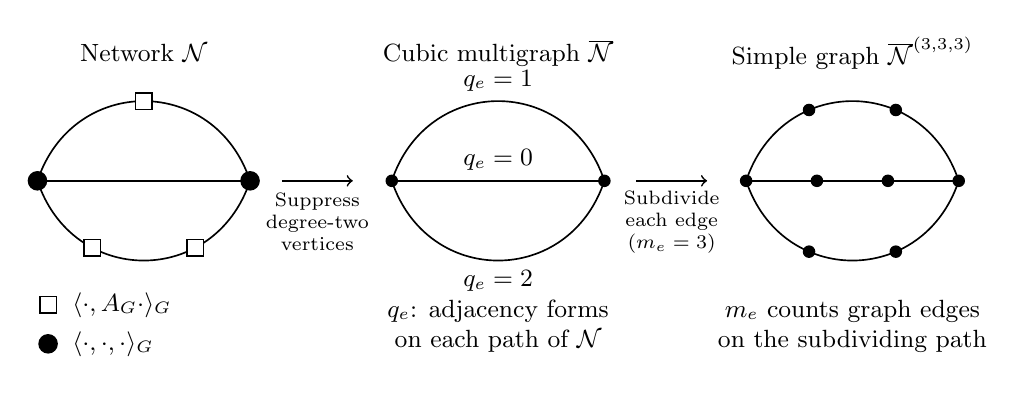
\begin{tikzpicture}[
  x=.9cm,y=.9cm,
  tensor/.style={circle,fill=black,inner sep=2.5pt},
  adjacency/.style={rectangle,draw,fill=white,minimum size=6pt,inner sep=0pt},
  vertex/.style={circle,fill=black,inner sep=1.6pt},
  every node/.style={font=\small},
  line width=.6pt,
]
\node at (1.5,1.8) {Network $\mathcal N$};
\draw (0,0)--(3,0);
\draw (0,0)..controls (.5,1.5) and (2.5,1.5)..(3,0)
  node[pos=.5,adjacency] {};
\draw (0,0)..controls (.5,-1.5) and (2.5,-1.5)..(3,0)
  node[pos=.3,adjacency] {} node[pos=.7,adjacency] {};
\node[tensor] at (0,0) {};
\node[tensor] at (3,0) {};
\node[adjacency] at (.15,-1.75) {};
\node[anchor=west] at (.35,-1.75) {$\langle\cdot,A_G\cdot\rangle_G$};
\node[tensor] at (.15,-2.3) {};
\node[anchor=west] at (.35,-2.3) {$\langle\cdot,\cdot,\cdot\rangle_G$};

\draw[->] (3.45,0)--(4.45,0);
\node[align=center,font=\scriptsize] at (3.95,-.58) {Suppress\\degree-two\\vertices};
\begin{scope}[xshift=4.5cm]
  \node at (1.5,1.8) {Cubic multigraph $\overline{\mathcal N}$};
  \draw (0,0)--(3,0) node[midway,above] {$q_e=0$};
  \draw (0,0)..controls (.5,1.5) and (2.5,1.5)..(3,0)
    node[midway,above] {$q_e=1$};
  \draw (0,0)..controls (.5,-1.5) and (2.5,-1.5)..(3,0)
    node[midway,below] {$q_e=2$};
  \node[vertex] at (0,0) {};
  \node[vertex] at (3,0) {};
  \node[align=center] at (1.5,-2.05) {$q_e$: adjacency forms\\on each path of $\mathcal N$};
\end{scope}

\draw[->] (8.45,0)--(9.45,0);
\node[align=center,font=\scriptsize] at (8.95,-.58) {Subdivide\\each edge\\($m_e=3$)};
\begin{scope}[xshift=9cm]
  \node at (1.5,1.8) {Simple graph $\overline{\mathcal N}^{(3,3,3)}$};
  \draw (0,0)--(3,0) node[pos=.333,vertex] {} node[pos=.667,vertex] {};
  \draw (0,0)..controls (.5,1.5) and (2.5,1.5)..(3,0)
    node[pos=.333,vertex] {} node[pos=.667,vertex] {};
  \draw (0,0)..controls (.5,-1.5) and (2.5,-1.5)..(3,0)
    node[pos=.333,vertex] {} node[pos=.667,vertex] {};
  \node[vertex] at (0,0) {};
  \node[vertex] at (3,0) {};
  \node[align=center] at (1.5,-2.05) {$m_e$ counts graph edges\\on the subdividing path};
\end{scope}
\end{tikzpicture}
\caption{A network, its cubic multigraph, and one simple subdivision.
The path represented by $e$ has $q_e$ adjacency forms and $q_e+1$ edges in $\mathcal N$;
a direct edge has $q_e=0$.
The subdivision on the right is chosen independently of the network paths,
with $m_e=3$ on every edge.
The expansions of $\val_G(\mathcal N)$ and $\hom(\overline{\mathcal N}^{\mathbf m},G)$
use the same coefficients $c_G(\overline{\mathcal N},\ell)$, with weights
$\prod_e\ell(e)^{q_e}$ and $\prod_e\ell(e)^{m_e}$, respectively.
Varying the lengths $m_e\geq3$ determines these coefficients and hence
the network value for every choice of $q_e\geq0$.}
\label{fig:network-subdivision}
\end{figure}


We next show that adjacency-image equivalence implies isomorphism for
graphs of nullity at most one.
For a graph $G$, we extend an orthonormal eigenbasis of $W_G$ to an
orthonormal eigenbasis $(u_i)_{i\in I}$ of $\R^{V(G)}$.
Let $\lambda_i$ be the eigenvalue of $u_i$ for each $i\in I$,
and let $I^{*}=\{i\in I:\lambda_i\ne0\}$.
Let $\gamma_1$ and $\gamma_3$ be the coefficient arrays of the
linear and trilinear forms in this eigenbasis, given by
\begin{equation}
  \label{eq:tensors}
  \begin{aligned}
  \gamma_1(i)&=\langle u_i\rangle_G, &
  \gamma_3(i,j,k)&=\langle u_i,u_j,u_k\rangle_G
  \end{aligned}
\end{equation}
for $i,j,k\in I$. For $x\in V(G)$, let $r_x=(u_i(x))_{i\in I}\in\R^I$ be
the row of $x$. These rows form an orthonormal basis of $\R^I$.
For $r\in\R^I$, let $r^{\otimes3}$ denote the array with entries
$r(i)r(j)r(k)$ for $i,j,k\in I$.
The rows satisfy
\begin{equation}
  \label{eq:rows}
  \begin{aligned}
  \gamma_3 &= \sum_{x \in V(G)} r_x^{\otimes 3}, &
  A_G(x,y) &= \sum_{i \in I} \lambda_i r_x(i) r_y(i).
  \end{aligned}
\end{equation}
We write $\gamma_3^{*}$ for the restriction of $\gamma_3$ to
indices in $I^{*}$.
In the eigenbasis $(u_i)_{i\in I^*}$ of $W_G$, the form
$\langle\cdot,\cdot,\cdot\rangle_G$ has coefficient array $\gamma_3^*$.
When $G$ has nullity one, we index the basis so that $I=I^*\sqcup\{0\}$
and $u_0$ spans $\ker A_G$.
In particular, $\gamma_1(0)=\sum_{x\in V(G)}u_0(x)$.
For such a graph, let $\tilde{r}_x=(u_i(x))_{i\in I^*}$ be
its reduced row at $x$.
Since $\tilde{r}_x$ is $r_x$ with its kernel coordinate omitted,
orthonormality of the rows gives
\begin{equation}\label{eq:gram}
 \langle\tilde{r}_x,\tilde{r}_y\rangle=\delta_{xy}-u_0(x)u_0(y).
\end{equation}
The coefficients of $\gamma_3$ outside
$\gamma_3^*$ are the $\gamma_3(i,j,k)$ with at least one
index equal to $0$.

If $G$ has nullity one and $|\supp u_0|>2$, then
\begin{equation}\label{eq:support-neighbourhoods}
 N_G(x)\ne N_G(y)\quad\text{for distinct }x,y\in\supp u_0.
\end{equation}
Indeed, for the standard coordinate vectors $e_x,e_y\in\R^{V(G)}$,
$e_x-e_y$ has support of size two, so it is not a scalar multiple of
$u_0$. Thus $A_G(e_x-e_y)\ne0$, which gives
\cref{eq:support-neighbourhoods}.

The final assertion of the next lemma is a special case of uniqueness of
orthogonal tensor decompositions~\cite[Theorem~3.2]{ZhangGolub2001}.
\begin{lemma}\label{lem:odeco}
 Let $X,I$ be finite sets, and let $R\in\R^{X\times I}$ be a matrix
 with orthonormal columns. Write $r_x\in\R^I$ for its row indexed by
 $x\in X$, and define $\kappa:\R^I\to\R$ by
 $\kappa(\xi)=\sum_{x\in X}\langle r_x,\xi\rangle^3$.
 Then
 \begin{equation}\label{eq:cubic-unit-rows}
  \{\xi:\lVert \xi\rVert=1,\ \kappa(\xi)=1\}
  =\{r_x:\lVert r_x\rVert=1\}.
 \end{equation}
 In particular, if $(r_x)_{x\in X}$ and $(r'_y)_{y\in Y}$ are
 orthonormal bases of the same Euclidean space and
 $\sum_x r_x^{\otimes3}=\sum_y(r'_y)^{\otimes3}$, then there is a
 bijection $\pi:X\to Y$ with $r'_{\pi(x)}=r_x$ for every $x\in X$.
\end{lemma}
\begin{proof}
 Let $\xi$ be a unit vector and put $c=R\xi$.
 Since the columns of $R$ are orthonormal, we have $\sum_xc_x^2=1$. Hence
 \begin{equation}\label{eq:cubic-unit-defect}
  1-\kappa(\xi)=\sum_x c_x^2(1-c_x)\geq0.
 \end{equation}
 Equality holds exactly when $c=e_x$ for some $x$,
 where $e_x$ is the standard coordinate vector.
 Then $\xi=R^{\top}c=r_x$.
 Conversely, if $\lVert r_x\rVert=1$, then $Rr_x$ is a unit vector
 whose $x$-coordinate is $1$, so $Rr_x=e_x$ and
 $\kappa(r_x)=1$. This proves \cref{eq:cubic-unit-rows}.
 The final assertion follows because equal cubic tensors identify the
 same set of unit rows.
\end{proof}
\begin{lemma}\label{lem:four-vertex-reconstruction}
Let $G,G'$ have nullity one and orthonormal eigenbases
$(u_i)_{i\in I}$ and $(u'_i)_{i\in I}$, respectively, with the same
corresponding eigenvalues $\lambda_i$.
Index both bases by $I=I^*\sqcup\{0\}$, with kernel vectors $u_0,u'_0$,
and write $\tilde{r}_x,\tilde{r}'_y\in\R^{I^*}$ for the reduced rows.
Suppose that $|\supp u_0|=|\supp u'_0|=4$ and
$\sum_xu_0(x)=\sum_yu'_0(y)=0$.
Suppose also that the reduced rows outside these supports agree as multisets and
$\sum_{x\in\supp u_0}\tilde{r}_x=\sum_{y\in\supp u'_0}\tilde{r}'_y$.
Then the reduced rows on the two supports agree as multisets.
\end{lemma}
\begin{proof}
  The rows outside each support are orthonormal by \cref{eq:gram}.
  We relabel the vertices of $G'$ outside $\supp u'_0$ so that
  $\tilde{r}'_z=\tilde{r}_z$ for every $z\notin\supp u_0$.
  We first show that $\supp u_0$ admits at least two distinct
  partitions into pairs on which $u_0$ sums to zero.
  For $w\in V(G)$, let $N_0(w)=N_G(w)\cap\supp u_0$.
  Then $\sum_{x\in N_0(w)}u_0(x)=(A_Gu_0)(w)=0$.
  If a nonempty proper subset $T$ of $\supp u_0$ satisfies
  $\sum_{x\in T}u_0(x)=0$, then $|T|=2$ and
  $\sum_{x\in\supp u_0\setminus T}u_0(x)=0$, since the four support
  entries are nonzero and sum to zero.
  Choose distinct $x,y\in\supp u_0$.
  By \cref{eq:support-neighbourhoods}, there is a vertex $w_1$ for which
  $N_0(w_1)$ contains exactly one of $x,y$.
  Thus $N_0(w_1)$ is nonempty and proper, and
  $\{N_0(w_1),\supp u_0\setminus N_0(w_1)\}$ is a first partition
  into zero-sum pairs.
  The two vertices of $N_0(w_1)$ also have different neighbourhoods,
  so there is a vertex $w_2$ for which $N_0(w_2)$ contains exactly
  one of them. Again $N_0(w_2)$ is nonempty and proper, so
  $\{N_0(w_2),\supp u_0\setminus N_0(w_2)\}$ is a partition into
  zero-sum pairs. It differs from the first partition because its
  two pairs separate the vertices of $N_0(w_1)$.

  We label $\supp u_0=\{a,b,c,d\}$ so that $u_0$ sums to zero
  on each pair in the two partitions
  $\{\{a,c\},\{b,d\}\}$ and $\{\{a,d\},\{b,c\}\}$.
  Since $u_0$ sums to zero on each of $\{a,c\}$, $\{a,d\}$ and
  $\{b,c\}$, we have
  $u_0(c)=u_0(d)=-u_0(a)=-u_0(b)$.
  Since $u_0$ is a unit vector, a choice of sign gives
  \begin{equation}
    \label{eq:support4}
    \begin{aligned}
      u_0(a)&=u_0(b)=\frac12, &
      u_0(c)&=u_0(d)=-\frac12.
    \end{aligned}
  \end{equation}
  Every $N_0(w)$ is then empty, equal to $\supp u_0$, or one of
  $\{a,c\}$, $\{a,d\}$, $\{b,c\}$, $\{b,d\}$.
  Since $\sum_yu'_0(y)=0$ and $|\supp u'_0|=4$, the same argument
  gives the nonzero entries $(\tfrac12,\tfrac12,-\tfrac12,-\tfrac12)$
  for $u'_0$, up to permutation and a choice of sign.

  We now show that $\{\tilde{r}_x:x\in\supp u_0\}$ and
  $\{\tilde{r}'_y:y\in\supp u'_0\}$ have the same centre and span the
  same affine plane.
  We choose the sign of $u'_0$ and label
  $\supp u'_0=\{a',b',c',d'\}$ so that
  $(u'_0(a'),u'_0(b'),u'_0(c'),u'_0(d'))=$
  $(\tfrac12,\tfrac12,-\tfrac12,-\tfrac12)$.
  Let $\sigma = \tilde{r}_a + \tilde{r}_b$,
  $f = (\tilde{r}_a - \tilde{r}_b)/\sqrt{2}$ and
  $g = (\tilde{r}_c - \tilde{r}_d)/\sqrt{2}$.
  Let $\sigma',f',g'$ be given by the formulas for $\sigma,f,g$ with
  primed vertices and rows.
  By \cref{eq:gram} and
  \cref{eq:support4}, the vectors $\sigma,f,g$ together with
  $(\tilde{r}_z)_{z\in V(G)\setminus\supp u_0}$ form an orthonormal basis of
  $\R^{I^*}$. Since $u_0$ is orthogonal to every $u_i$ with $i\in I^*$,
  we have $\sum_xu_0(x)\tilde{r}_x=0$.
  Substituting \cref{eq:support4} gives
  $\tilde{r}_a+\tilde{r}_b=\tilde{r}_c+\tilde{r}_d$, so $\sigma=\tilde{r}_c+\tilde{r}_d$. Hence
  \begin{equation}
    \label{eq:special-rows}
    \begin{aligned}
    \tilde{r}_a &= \frac{1}{2} \sigma + \frac{1}{\sqrt{2}} f, &
    \tilde{r}_b &= \frac{1}{2} \sigma - \frac{1}{\sqrt{2}} f, &
    \tilde{r}_c &= \frac{1}{2} \sigma + \frac{1}{\sqrt{2}} g, &
    \tilde{r}_d &= \frac{1}{2} \sigma - \frac{1}{\sqrt{2}} g.
    \end{aligned}
  \end{equation}
  The centres of $\{\tilde{r}_a,\tilde{r}_b,\tilde{r}_c,\tilde{r}_d\}$ and
  $\{\tilde{r}'_{a'},\tilde{r}'_{b'},\tilde{r}'_{c'},\tilde{r}'_{d'}\}$ are their averages
  $\sigma/2$ and $\sigma'/2$. By the assumed equality of the support-row sums,
  \begin{equation}\label{eq:quartet-offset}
    \frac12\sigma'=\frac14\sum_{y\in\supp u'_0}\tilde{r}'_y
    =\frac14\sum_{x\in\supp u_0}\tilde{r}_x=\frac12\sigma.
  \end{equation}
  Since $\sigma'=\sigma$ and $\tilde{r}'_z=\tilde{r}_z$ for
  $z\notin\supp u_0$, the orthonormal bases
  $\{\sigma,f,g\}\cup\{\tilde{r}_z:z\notin\supp u_0\}$ and
  $\{\sigma',f',g'\}\cup\{\tilde{r}'_z:z\notin\supp u'_0\}$ give
  \begin{equation}\label{eq:quartet-plane}
   \spn(f,g)
   =\spn\bigl(\{\tilde{r}_z:z\notin\supp u_0\}\cup\{\sigma\}\bigr)^\perp
   =\spn(f',g').
  \end{equation}
  Thus both sets of four vectors have affine span $\sigma/2+\spn(f,g)$.

  We now use the entries of $A_{G'}$ to show that $f'\in\{\pm f,\pm g\}$.
  Let $\alpha,\beta\in\R$ be the coefficients in $f'=\alpha f+\beta g$.
  Since $(f,g)$ is orthonormal and $f'$ is a unit vector,
  $\alpha^2+\beta^2=1$.
  For each $z\in V(G)\setminus\supp u_0$, let
  $\Delta_z^f=A_G(a,z)-A_G(b,z)$ and
  $\Delta_z^g=A_G(c,z)-A_G(d,z)$.
  By \cref{eq:rows,eq:special-rows},
  \begin{equation}\label{eq:quartet-adjacency}
    \begin{aligned}
      \sqrt2 f^{\top}\diag(\lambda_i)_{i\in I^*}\tilde{r}_z &= \Delta_z^f,\\
      \sqrt2 g^{\top}\diag(\lambda_i)_{i\in I^*}\tilde{r}_z &= \Delta_z^g,\\
      \sigma^{\top}\diag(\lambda_i)_{i\in I^*}\tilde{r}_z &= A_G(a,z)+A_G(b,z).
    \end{aligned}
  \end{equation}
  Since $\sigma'=\sigma$ and $f'=\alpha f+\beta g$, we have
  $\tilde{r}'_{a'}=\tfrac12\sigma+\tfrac1{\sqrt2}(\alpha f+\beta g)$
  by \cref{eq:special-rows} for $G'$.
  Substituting this formula for $\tilde{r}'_{a'}$ and $\tilde{r}'_z=\tilde{r}_z$ into
  the second identity in \cref{eq:rows} for $G'$, and using
  \cref{eq:quartet-adjacency}, gives
  \begin{equation}
    \label{eq:integrality}
    A_{G'}(a', z) = \frac{1}{2}\bigl(A_G(a,z)+A_G(b,z)\bigr)
      + \frac{1}{2}(\alpha\Delta_z^f+\beta\Delta_z^g)\in\{0,1\}.
  \end{equation}

  We have $\alpha\beta=0$ whenever a vertex $z\notin\supp u_0$ satisfies
  \begin{equation}\label{eq:quartet-probe}
    A_G(a,z)+A_G(b,z)=A_G(c,z)+A_G(d,z)=1.
  \end{equation}
  Indeed, then $\Delta_z^f,\Delta_z^g\in\{\pm1\}$ and
  $A_G(a,z)+A_G(b,z)=1$, so \cref{eq:integrality} gives
  $\alpha\Delta_z^f+\beta\Delta_z^g=\pm1$.
  Squaring gives
  $1=\alpha^2+\beta^2+2\alpha\beta\Delta_z^f\Delta_z^g
  =1+2\alpha\beta\Delta_z^f\Delta_z^g$, so $\alpha\beta=0$.
  \Cref{fig:quartet-geometry} gives a geometric interpretation of this calculation.

  \begin{figure}[tb]
\centering
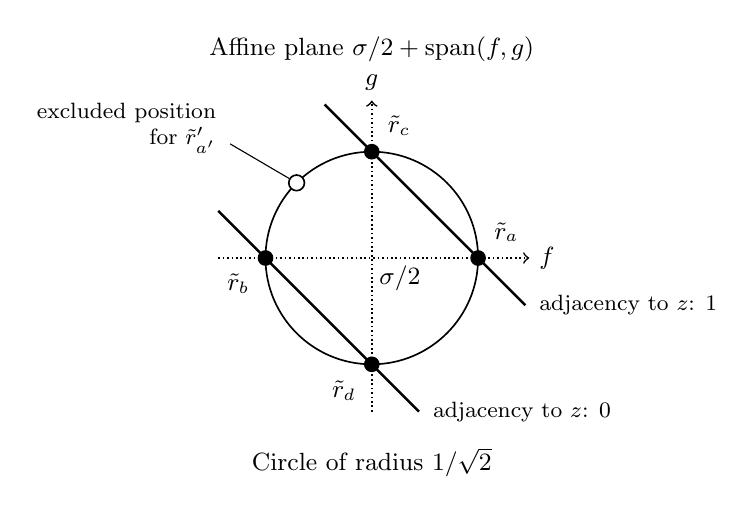
\begin{tikzpicture}[
  every node/.style={font=\small},
  point/.style={circle,fill=black,inner sep=2pt},
  candidate/.style={circle,draw,fill=white,inner sep=2pt},
  line width=.6pt,
]
\node at (0,2.65) {Affine plane $\sigma/2+\spn(f,g)$};
\draw[densely dotted,->] (-1.95,0)--(2,0) node[right] {$f$};
\draw[densely dotted,->] (0,-1.95)--(0,2) node[above] {$g$};
\draw (0,0) circle[radius=1.35];
\draw[line width=.9pt] (-.6,1.95)--(1.95,-.6);
\node[anchor=west,font=\footnotesize] at (2,-.6) {adjacency to $z$: $1$};
\draw[line width=.9pt] (-1.95,.6)--(.6,-1.95);
\node[anchor=west,font=\footnotesize] at (.65,-1.95) {adjacency to $z$: $0$};
\node[fill=white,inner sep=1pt,anchor=north west] at (.05,-.05) {$\sigma/2$};
\node[point,label=above right:$\tilde{r}_a$] at (1.35,0) {};
\node[point,label=below left:$\tilde{r}_b$] at (-1.35,0) {};
\node[point,label=above right:$\tilde{r}_c$] at (0,1.35) {};
\node[point,label=below left:$\tilde{r}_d$] at (0,-1.35) {};
\node[candidate] (excluded) at (135:1.35) {};
\node[anchor=east,align=right,font=\footnotesize] at (-1.85,1.65)
  {excluded position\\for $\tilde{r}'_{a'}$};
\draw[thin] (-1.8,1.45)--(excluded);
\node at (0,-2.6) {Circle of radius $1/\sqrt2$};
\end{tikzpicture}
\caption{Geometric interpretation of the calculation giving $\alpha\beta=0$.
The figure assumes that $z\in V(G)\setminus\supp u_0$ is adjacent to $a,c$
and not to $b,d$; the other cases of \cref{eq:quartet-probe} are symmetric.
For a candidate $\tilde{r}'_{a'}=\sigma/2+(\alpha f+\beta g)/\sqrt2$,
the circle gives $\alpha^2+\beta^2=1$.
By \cref{eq:integrality}, the two lines have equations
$\alpha+\beta=1$ and $\alpha+\beta=-1$.
Squaring either equation and subtracting the circle equation gives
$2\alpha\beta=0$. The hollow point is on the circle but off both lines,
so \cref{eq:integrality} excludes it.}
\label{fig:quartet-geometry}
\end{figure}


  We show that \cref{eq:quartet-probe} holds for some
  $z\in V(G)\setminus\supp u_0$. Otherwise, the list of
  possible sets $N_0(z)$ implies
  $N_0(z)\in\{\varnothing,\supp u_0\}$ for every
  $z\notin\supp u_0$.
  For $w\in\supp u_0$, we have $w\notin N_0(w)$ because $G$ has no loops.
  Thus a nonempty $N_0(w)$ must be one of
  $\{a,c\}$, $\{a,d\}$, $\{b,c\}$ and $\{b,d\}$.
  Every nonisolated vertex in the graph induced by $\supp u_0$
  therefore has exactly two neighbours, one in $\{a,b\}$ and one in
  $\{c,d\}$. A nonisolated vertex in $\{a,b\}$ is adjacent to the
  other vertex of $\{a,b\}$; the same holds for $\{c,d\}$.
  If the induced graph has an edge, it therefore also has an edge
  between $\{a,b\}$ and $\{c,d\}$.
  Each of these two sets then contains a nonisolated vertex and hence
  both its vertices are nonisolated. All four vertices have degree two,
  so the induced graph is a cycle of length four.
  Thus either the induced graph is edgeless, or it is a four-cycle.
  There are distinct $x,y\in\supp u_0$ with $N_0(x)=N_0(y)$:
  any two vertices in the edgeless case, or opposite vertices in the
  four-cycle case. Also
  $N_G(x)\setminus\supp u_0=N_G(y)\setminus\supp u_0$, because every
  vertex outside the support is adjacent to all four support vertices
  or to none. Hence $N_G(x)=N_G(y)$, contradicting
  $N_G(x)\ne N_G(y)$ for distinct $x,y\in\supp u_0$.

  A vertex $z\notin\supp u_0$ satisfying \cref{eq:quartet-probe}
  exists, so $\alpha\beta=0$. Together with $\alpha^2+\beta^2=1$,
  this gives $(\alpha,\beta)\in\{(1,0),(-1,0),(0,1),(0,-1)\}$,
  hence $f'\in\{\pm f,\pm g\}$. Since $(f',g')$ is orthonormal in
  $\spn(f,g)$, we have $\{\pm f',\pm g'\}=\{\pm f,\pm g\}$.
  Together with $\sigma'=\sigma$, \cref{eq:special-rows} now gives
  \begin{equation}\label{eq:quartet-row-equality}
    \{\tilde{r}_a,\tilde{r}_b,\tilde{r}_c,\tilde{r}_d\}
    =\{\tilde{r}'_{a'},\tilde{r}'_{b'},\tilde{r}'_{c'},\tilde{r}'_{d'}\}.
  \end{equation}
  The four vectors on each side are distinct by \cref{eq:special-rows},
  so they agree as multisets.
\end{proof}

\begin{lemma}\label{lem:reconstruction}
 Let $G$ have nullity at most one, and let $G'$ be a graph.
 If $G\sim_{\mathrm{im}}G'$, then $G\cong G'$.
\end{lemma}
\begin{proof}
  We fix a bijective linear map $U:W_G\to W_{G'}$ witnessing
  $G\sim_{\mathrm{im}}G'$.
  The graphs $G$ and $G'$ have the same number of vertices because
  $G\sim_{\mathrm{im}}G'$. The map $U$ intertwines
  $A_G|_{W_G}$ with $A_{G'}|_{W_{G'}}$, so their nonzero eigenvalues agree
  with multiplicities. Thus their zero multiplicities also agree,
  and both graphs have the same nullity, at most one.
  We fix an orthonormal eigenbasis
  $(u_i)_{i\in I}$ of $\R^{V(G)}$.
  Let $(u'_i)_{i\in I}$ be an orthonormal eigenbasis of $\R^{V(G')}$
  with $u'_i=Uu_i$ for every $i\in I^*$.
  Then $u_i$ and $u'_i$ have the same eigenvalue $\lambda_i$ for every
  $i\in I$. We use primes for quantities associated with $G'$.
  By \cref{eq:adjacency-image-equivalence} and
  \cref{eq:image-sum-transport}, for $i,j,k\in I^*$,
  \begin{equation}\label{eq:transported-tensors}
    \begin{aligned}
      \gamma'_1(i)&=\langle Uu_i\rangle_{G'}
        =\langle u_i\rangle_G=\gamma_1(i),\\
      \gamma'_3(i,j,k)&=\langle Uu_i,Uu_j,Uu_k\rangle_{G'}
        =\langle u_i,u_j,u_k\rangle_G=\gamma_3(i,j,k).
    \end{aligned}
  \end{equation}
  For $x\in V(G)$ and $y\in V(G')$, let
  $\tilde{r}_x=(u_i(x))_{i\in I^*}$ and
  $\tilde{r}'_y=(u'_i(y))_{i\in I^*}$ be the reduced rows.
  A bijection $\pi:V(G)\to V(G')$ with $\tilde{r}'_{\pi(x)}=\tilde{r}_x$ is a
  graph isomorphism. The zero-eigenvalue terms in the second identity of
  \cref{eq:rows} vanish, so for $x,y\in V(G)$ we have
  \begin{equation}\label{eq:row-isomorphism}
    A_{G'}(\pi(x),\pi(y))
    =\sum_{i\in I^*}\lambda_i\tilde{r}'_{\pi(x)}(i)\tilde{r}'_{\pi(y)}(i)
    =\sum_{i\in I^*}\lambda_i\tilde{r}_x(i)\tilde{r}_y(i)=A_G(x,y).
  \end{equation}
  If $\gamma_3=\gamma'_3$, then by \cref{lem:odeco} there is a
  bijection $\pi$ with $r'_{\pi(x)}=r_x$, hence $\tilde{r}'_{\pi(x)}=\tilde{r}_x$.
  If the graphs are nonsingular, then $I^*=I$, so
  \cref{eq:transported-tensors} already gives $\gamma_3=\gamma'_3$
  and hence $G\cong G'$.

  We therefore assume that both graphs have nullity one.
  We index $(u_i)$ and $(u'_i)$ so that $I=I^*\sqcup\{0\}$, with unit kernel
  vectors $u_0,u'_0$. Once $(u_i)_{i\in I^*}$ and $(u'_i)_{i\in I^*}$ are fixed,
  the only remaining choices are the signs of $u_0$ and $u'_0$.
  We first compare the coefficients involving index $0$, which are
  not compared in \cref{eq:transported-tensors}.
  By symmetry of $\gamma_3$, the \emph{missing coefficients} are
  $\gamma_1(0)$, $\gamma_3(0,0,0)$, $\gamma_3(0,0,k)$ and
  $\gamma_3(0,j,k)$ for $j,k\in I^*$.
  We seek a choice of signs for $u_0,u'_0$ for which these coefficients
  agree with their primed counterparts. If these coefficients agree, then
  \cref{eq:transported-tensors} gives $\gamma_3=\gamma'_3$,
  and \cref{lem:odeco} gives a vertex bijection $\pi$ satisfying
  $\tilde{r}'_{\pi(v)}=\tilde{r}_v$ for every $v\in V(G)$.
  Replacing $u_0$ by $-u_0$ negates $\gamma_1(0)$,
  $\gamma_3(0,0,0)$ and $\gamma_3(0,j,k)$, while leaving
  $\gamma_3(0,0,k)$ unchanged. Replacing $u'_0$ by $-u'_0$
  has the same effect on the primed coefficients.

  The arrays $\gamma_1,\gamma_3$ satisfy the following identities for all $i,j,k,l\in I$
  because the vectors $r_x$ form an orthonormal basis:
  \begin{gather}
    \label{eq:id-norm}
    \sum_{m \in I} \gamma_1(m)^{2} = |V(G)|, \\
    \label{eq:id-unit}
    \sum_{m \in I} \gamma_1(m) \gamma_3(m,j,k) = \delta_{jk}, \\
    \label{eq:id-trace}
    \sum_{m \in I} \gamma_3(j,m,m) = \gamma_1(j), \\
    \label{eq:id-assoc}
    \sum_{m \in I} \gamma_3(i,j,m) \gamma_3(m,k,l)
      = \sum_{x \in V(G)} u_i(x) u_j(x) u_k(x) u_l(x).
  \end{gather}
  Separating the term $m=0$ in \cref{eq:id-trace} gives, for $k\in I^*$,
  \begin{equation}
    \label{eq:trace-completion}
    \begin{aligned}
      \gamma_3(0,0,k) &= \gamma_1(k) - \sum_{i\in I^*}\gamma_3(k,i,i),\\
      \gamma_3(0,0,0) &= \gamma_1(0) - \sum_{i\in I^*}\gamma_3(0,i,i).
    \end{aligned}
  \end{equation}
  The first identity involves only coefficients at indices in $I^*$ on
  the right-hand side, so $\gamma'_3(0,0,k)=\gamma_3(0,0,k)$ by
  \cref{eq:transported-tensors}. The second determines
  $\gamma_3(0,0,0)$ from $\gamma_1(0)$ and the coefficients
  $\gamma_3(0,j,k)$. Thus agreement of all missing coefficients
  reduces to agreement of $\gamma_1(0)$ and $\gamma_3(0,j,k)$
  with their primed counterparts.

  For the case analysis, let $\mathsf C_0$ be the symmetric
  $I^*\times I^*$ matrix defined by
  \begin{equation}\label{eq:unknowns}
    \mathsf C_0(j,k) = \gamma_3(0,j,k).
  \end{equation}
  Separating the term $m=0$ in \cref{eq:id-norm} gives
  $\gamma_1(0)^2=|V(G)|-\sum_{i\in I^*}\gamma_1(i)^2$, so
  $\gamma_1(0)^2=(\gamma'_1(0))^2$ by \cref{eq:transported-tensors}.
  We divide the remaining proof into $\gamma_1(0)\ne0$ (Case A)
  and $\gamma_1(0)=0$ (Case B).
  Within Case B, we distinguish $\rank\mathsf C_0\geq3$ (Case B1)
  from $\rank\mathsf C_0\leq2$ (Case B2).
  In Cases A and B1, we show that a choice of sign for $u'_0$ gives
  $\gamma'_1(0)=\gamma_1(0)$ and $\mathsf C'_0=\mathsf C_0$.
  In Case B2, we use the graph structure to show that $u_0$ has
  support of size two or four. In both subcases, we show directly
  that $(\tilde{r}_x)_{x\in V(G)}$ and $(\tilde{r}'_y)_{y\in V(G')}$ agree as multisets.

  \emph{Case A: $\gamma_1(0) \neq 0$.} We choose the sign of $u'_0$ so
  that $\gamma'_1(0)=\gamma_1(0)$. Separating the term $m=0$ in
  \cref{eq:id-unit} gives
  \begin{equation}
    \label{eq:caseA}
    \gamma_1(0) \mathsf{C}_0(j,k) = \delta_{jk} - \sum_{i \in I^{*}} \gamma_1(i) \gamma_3(i,j,k).
  \end{equation}
  The right-hand side for $G'$ equals the right-hand side for $G$ by
  \cref{eq:transported-tensors}, and dividing by
  $\gamma_1(0)=\gamma'_1(0)\neq0$ gives $\mathsf C'_0=\mathsf C_0$.
  Hence $\gamma_3=\gamma'_3$.

  \emph{Case B: $\gamma_1(0) = 0$.} Then $\gamma'_1(0)=0$, since
  $(\gamma'_1(0))^2=\gamma_1(0)^2$. Here \cref{eq:id-unit} no longer
  determines $\mathsf C_0$.

  \emph{Case B1: $\rank \mathsf{C}_0 \geq 3$.} We show that
  $\mathsf C'_0=\pm\mathsf{C}_0$ by comparing their $2\times2$ minors.
  For $i,j,k,l \in I^{*}$ let $Q(i,j;k,l)$ be the sum of the terms with
  $m\neq0$ in \cref{eq:id-assoc},
  \begin{equation}\label{eq:q-tensor}
   Q(i,j;k,l) = \sum_{m \in I^{*}} \gamma_3(i,j,m) \gamma_3(m,k,l),
  \end{equation}
  which involves only $\gamma_3^*$.
  Separating the term $m=0$ in \cref{eq:id-assoc} gives
  \begin{equation}
    \label{eq:assoc-split}
    \mathsf{C}_0(i,j)\mathsf{C}_0(k,l)+Q(i,j;k,l)
    =\sum_{x \in V(G)} u_i(x) u_j(x) u_k(x) u_l(x).
  \end{equation}
  The right-hand side is symmetric in $(i,j,k,l)$, so subtracting from
  \cref{eq:assoc-split} the same identity with $j$ and $k$ exchanged
  gives
  \begin{equation}
    \label{eq:minors}
    \mathsf{C}_0(i,j) \mathsf{C}_0(k,l) - \mathsf{C}_0(i,k) \mathsf{C}_0(j,l) = Q(i,k;j,l) - Q(i,j;k,l).
  \end{equation}
  The left-hand side is the minor of $\mathsf{C}_0$ with rows $i,l$ and
  columns $j,k$. The right-hand side involves only $\gamma_3^*$,
  which $G$ and $G'$ share by \cref{eq:transported-tensors}. Hence each
  $2\times2$ minor of $\mathsf C'_0$ equals the minor of
  $\mathsf{C}_0$ with the same rows and columns.
  Thus the exterior squares of $\mathsf C_0$ and $\mathsf C'_0$ are equal.
  Since $\rank\mathsf C_0\geq3$, \cite[Corollary~4.1]{Greenhill1999}
  gives $\mathsf C'_0=\pm\mathsf C_0$.
  We choose the sign of $u'_0$ so that $\mathsf C'_0=\mathsf{C}_0$.
  Hence $\gamma_3=\gamma'_3$.

  \emph{Case B2: $\rank \mathsf{C}_0 \leq 2$.} We show that
  $\{\tilde{r}_z:z\notin\supp u_0\}=\{\tilde{r}'_z:z\notin\supp u'_0\}$.
  Let $R$ be the matrix with rows $\tilde{r}_x$. Its columns are
  orthonormal, and \cref{eq:gram} gives
  $\lVert\tilde{r}_x\rVert^2=1-u_0(x)^2$.
  Thus $\tilde{r}_x$ is a unit vector exactly when $x\notin\supp u_0$.
  The same holds for $\tilde{r}'_y$ and $\supp u'_0$.
  Let $\kappa$ and $\kappa'$ be the cubic forms with coefficient
  arrays $\gamma_3^*$ and $(\gamma'_3)^*$, respectively, so
  \begin{equation}\label{eq:reduced-cubic}
   \kappa(\xi)=\sum_x\langle\tilde{r}_x,\xi\rangle^3
   =\sum_y\langle\tilde{r}'_y,\xi\rangle^3=\kappa'(\xi)
  \end{equation}
  by \cref{eq:transported-tensors}.
  By \cref{lem:odeco} and \cref{eq:reduced-cubic},
  \begin{equation}\label{eq:outside-rows}
   \{\tilde{r}_z:z\notin\supp u_0\}
   =\{\xi:\lVert \xi\rVert=1,\ \kappa(\xi)=1\}
   =\{\tilde{r}'_z:z\notin\supp u'_0\}.
  \end{equation}
  Each of these row families is orthonormal by \cref{eq:gram}, so its
  members are distinct. Since $G$ and $G'$ have the same number of
  vertices, \cref{eq:outside-rows} also gives
  $|\supp u'_0|=|\supp u_0|$.
  We relabel the vertices of $G'$ outside $\supp u'_0$ so that
  $\tilde{r}'_z=\tilde{r}_z$ for every $z\notin\supp u_0$.

  It remains to compare $(\tilde{r}_x)_{x\in\supp u_0}$ and
  $(\tilde{r}'_y)_{y\in\supp u'_0}$ as multisets.
  Their sums agree: by
  \cref{eq:transported-tensors} and \cref{eq:outside-rows},
  \begin{equation}\label{eq:support-row-sum}
    \sum_{x\in\supp u_0}\tilde{r}_x
    = (\gamma_1(i))_{i\in I^*}-\sum_{z\notin\supp u_0}\tilde{r}_z
    = \sum_{y\in\supp u'_0}\tilde{r}'_y.
  \end{equation}
  We claim that
  \begin{equation}\label{eq:kernel-support-sizes}
    |\supp u_0|\in\{2,4\}.
  \end{equation}
  Since $\mathsf{C}_0 = R^{\top} \diag(u_0) R$ and
  $\rank R=|V(G)|-1$, Sylvester's rank inequality gives
  $|\supp u_0| \leq \rank \mathsf{C}_0 + 2 \leq 4$.
  The support has at least two vertices because $u_0\ne0$ and
  $\gamma_1(0)=0$.
  Suppose it has three vertices. For every nonempty proper subset
  $T$ of $\supp u_0$, we have $\sum_{x\in T}u_0(x)\ne0$, since
  the three entries are nonzero and their sum is zero.
  The equation $(A_Gu_0)(w)=\sum_{x\in N_G(w)}u_0(x)=0$ therefore
  forces every vertex $w$ to be adjacent to all three support
  vertices or to none. Thus $N_G(x)=N_G(y)$ for any two distinct
  support vertices $x,y$, contradicting \cref{eq:support-neighbourhoods}.

  \emph{Case B2 with $|\supp u_0|=2$.} Write
  $\supp u_0=\{x,y\}$ and $\supp u'_0=\{x',y'\}$.
  Since $u_0(x)=-u_0(y)\ne0$, we have
  $0=\langle u_0,u_i\rangle_G=u_0(x)(u_i(x)-u_i(y))$ for all $i\in I^*$,
  so $\tilde{r}_x=\tilde{r}_y$. The same holds for $u'_0$.
  By \cref{eq:support-row-sum},
  $\tilde{r}_x+\tilde{r}_y=\tilde{r}'_{x'}+\tilde{r}'_{y'}$, hence
  $\tilde{r}_x=\tilde{r}_y=\tilde{r}'_{x'}=\tilde{r}'_{y'}$.
  Together with \cref{eq:outside-rows}, this gives a vertex bijection
  $\pi$ satisfying $\tilde{r}'_{\pi(v)}=\tilde{r}_v$ for every $v\in V(G)$.
  Hence $G\cong G'$ by \cref{eq:row-isomorphism}.

  \emph{Case B2 with $|\supp u_0|=4$.}
  Both kernel vectors have support of size four and sum zero.
  Their outside rows agree by \cref{eq:outside-rows}, and their
  support-row sums agree by \cref{eq:support-row-sum}.
  Thus \cref{lem:four-vertex-reconstruction} identifies the remaining
  reduced rows as multisets.
  Combining the two correspondences gives a bijection $\pi$ with
  $\tilde{r}'_{\pi(x)}=\tilde{r}_x$, which is an isomorphism by \cref{eq:row-isomorphism}.
\end{proof}

\begin{proof}[Proof of \cref{thm:main}]

 Suppose $G\equiv_{\mathcal D_3}G'$. By \cref{lem:characterisation},
 $G\sim_{\mathrm{im}}G'$. Hence $G\cong G'$ by \cref{lem:reconstruction}.
 Conversely, an isomorphism $\pi:G\to G'$ gives a bijection
 $\varphi\mapsto\pi\circ\varphi$ between homomorphisms $F\to G$ and $F\to G'$
 for every $F$, so $G\equiv_{\mathcal D_3}G'$.
 A graph with simple spectrum has nullity at most one, because a real
 symmetric matrix with pairwise distinct eigenvalues has zero as an
 eigenvalue at most once; hence $\mathcal D_3$ is complete on simple
 spectrum.
\end{proof}

\begin{remark}\label{rem:nullity-bound}
The nullity bound in \cref{thm:main} cannot be raised to three.
Let $B$ be the cricket graph shown in \cref{fig:cricket}.
The graphs $\CFI_0(B)$ and $\CFI_1(B)$ defined in
\cref{eq:ss-cfi-definition} each have $14$ vertices.
A direct calculation gives nullity three for both graphs.
They are non-isomorphic and homomorphism indistinguishable over
$\mathcal D_3$ by~\cite[Corollary~3.7 and the proof of Corollary~4.2]{Roberson2026}.
It remains open whether \cref{thm:main} extends to graphs of nullity two.
An exhaustive search found no pair of non-isomorphic graphs of nullity two
on at most $11$ vertices that are homomorphism indistinguishable over
$\mathcal D_3$.
\end{remark}

\begin{figure}[tb]
\centering
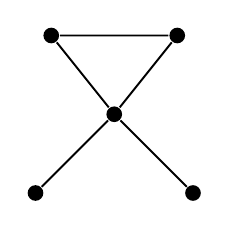
\begin{tikzpicture}[
  vertex/.style={circle,fill,inner sep=2pt},
  line width=.7pt,
]
\node[vertex] (centre) at (0,0) {};
\node[vertex] (upperleft) at (-.8,1) {};
\node[vertex] (upperright) at (.8,1) {};
\node[vertex] (lowerleft) at (-1,-1) {};
\node[vertex] (lowerright) at (1,-1) {};
\draw (centre)--(upperleft)--(upperright)--(centre);
\draw (lowerleft)--(centre)--(lowerright);
\end{tikzpicture}
\caption{The cricket graph $B$.}
\label{fig:cricket}
\end{figure}


\section{Proof of Proposition~\ref{prop:closure}}
\label{sec:restriction}

It suffices to prove the proposition for a subsequence of $(H_N)$.
If $\calF'\subseteq\calF$ is the class obtained from a subsequence and
$\equiv_{\calF'}$ coincides with $\equiv_{\mathcal D_3}$, then
$\equiv_{\calF}$ coincides with $\equiv_{\mathcal D_3}$ as well, because
$\calF'\subseteq\calF\subseteq\mathcal D_3$.
Every tail of $(H_N)$ still has unbounded clique-minor size, since a finite
initial segment has bounded clique-minor size. We can therefore choose
and reindex a subsequence so that $H_N$ contains $K_{3N}$ as
a minor for every $N\geq1$; \cref{lem:subdivision-containment} below uses this
property.
We use the subdivision notation $H^{\mathbf m}$ and the labelled
coefficients $c_G(H,\ell)$ from \cref{sec:characterisation}.
For this reindexed sequence, let $\calF'$ consist
of $K_1$ and the graphs $H_N^{\mathbf m}$ for all $N\geq1$ and all tuples $\mathbf m$.

\begin{lemma}\label{lem:subdivision-containment}
 Let $N\geq1$ and suppose that $H_N$ contains $K_{3N}$ as a minor.
 Let $H$ be a connected cubic multigraph with at most $N$ vertices.
 Then $H_N$ contains a subgraph isomorphic to a subdivision of $H$.
\end{lemma}
\begin{proof}
 Since a subdivision of a subdivision of $H$ is a subdivision of $H$, it
 suffices to find a simple subcubic subdivision $J$ of $H$ with at most
 $3N$ vertices. Such a $J$ is a subgraph of $K_{3N}$ and hence a
 minor of $H_N$. Since $J$ is subcubic, it is a topological minor
 of $H_N$~\cite[Section~1.7]{Diestel2017}, so $H_N$ contains a subgraph
 isomorphic to a subdivision of $J$ and hence to a subdivision of $H$.
 Let $J=H^{\mathbf m}$, where $m_e=3$ for each loop, $m_e=2$ for all
 but one edge in each group of parallel non-loop edges, and $m_e=1$
 for all other edges.
 Then $J$ is simple and subcubic. There are two new vertices for each
 loop and $k-1\leq2$ for each group of $k\geq2$ parallel non-loop edges.
 Since $H$ is cubic, these loops and parallel-edge groups have
 disjoint vertex sets. Hence $|V(J)|-|V(H)|\leq2|V(H)|\leq2N$,
 so $J$ has at most $3N$ vertices.
\end{proof}

\begin{lemma}\label{lem:independent-path-lengths}
 Let $H$ be a connected cubic multigraph and let $m\geq1$ be an integer.
 There is a connected cubic graph $D$ with the following property.
 If a graph $X$ contains a subgraph isomorphic to a subdivision of $D$,
 then there are an injection $\iota:V(H)\hookrightarrow V(X)$ and finite
 sets $Q_e\subseteq\Z_{\geq1}$ with $|Q_e|\geq m+1$ for each $e\in E(H)$
 such that, for every $\mathbf q\in\prod_eQ_e$, there is a subdivision
 of $H$ in $X$ with vertex map $\iota$ and paths $R_e$ of lengths $q_e+1$.
 Here $R_e$ is a cycle through $\iota(v)$ if $e$ is a loop at $v$.
 At least one edge of $X$ lies outside the chosen subdivision.
\end{lemma}
\begin{proof}
We construct $D$ by replacing each edge of $H$ by a chain of $m$ diamonds.
The \emph{diamond} $K_4-ab$ is $K_4$ on vertices $a,b,c,d$ with the
edge $ab$ deleted. Its vertices $a,b$ have degree two, and $c,d$ have
degree three. A chain consists of $m$ disjoint copies together with
an edge from $b$ in each copy to $a$ in the next.
For each edge $vw$ of $H$, take a separate chain and add edges from
$v$ to $a$ in its first copy and from $b$ in its last copy to $w$.
The resulting graph $D$ is connected and cubic.
\Cref{fig:diamond-objects} illustrates an example of the construction.
\begin{figure}[tb]
\centering
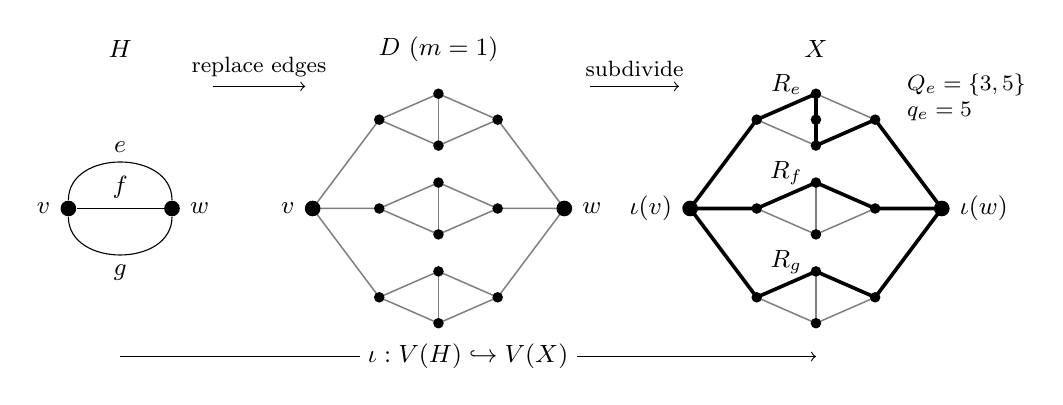
\begin{tikzpicture}[
  x=.94cm,y=.94cm,
  every node/.style={font=\small},
  vertex/.style={circle,fill=black,inner sep=1.35pt},
  branch/.style={circle,fill=black,inner sep=2pt},
  edge/.style={draw=black!50,line width=.55pt},
  chosen/.style={draw=black,line width=1.3pt},
]
\node at (0,2.15) {$H$};
\node at (4.3,2.15) {$D$ ($m=1$)};
\node at (9.4,2.15) {$X$};
\node[branch,label=left:$v$] (hu) at (-.7,0) {};
\node[branch,label=right:$w$] (hv) at (.7,0) {};
\draw (hu) .. controls (-.7,.8) and (.7,.8) .. (hv)
  node[midway,above] {$e$};
\draw (hu)--(hv) node[midway,above] {$f$};
\draw (hu) .. controls (-.7,-.8) and (.7,-.8) .. (hv)
  node[midway,below] {$g$};

\foreach \offset/\name in {4.3/d,9.4/x} {
  \begin{scope}[xshift=\offset*.94cm]
    \coordinate (\name u) at (-1.7,0);
    \coordinate (\name v) at (1.7,0);
    \foreach \height/\j in {1.2/e,0/f,-1.2/g} {
      \coordinate (\name a\j) at (-.8,\height);
      \coordinate (\name b\j) at (.8,\height);
      \coordinate (\name c\j) at (0,\height+.35);
      \coordinate (\name d\j) at (0,\height-.35);
      \draw[edge] (\name u)--(\name a\j)--(\name c\j)--(\name b\j)--(\name v);
      \draw[edge] (\name a\j)--(\name d\j)--(\name b\j);
      \draw[edge] (\name c\j)--(\name d\j);
    }
  \end{scope}
}
\node[branch,label=left:$v$] at (du) {};
\node[branch,label=right:$w$] at (dv) {};
\node[branch,label=left:$\iota(v)$] at (xu) {};
\node[branch,label=right:$\iota(w)$] at (xv) {};
\coordinate (xs) at (9.4,1.2);
\draw[chosen] (xu)--(xae)--(xce)--(xs)--(xde)--(xbe)--(xv);
\draw[chosen] (xu)--(xaf)--(xcf)--(xbf)--(xv);
\draw[chosen] (xu)--(xag)--(xcg)--(xbg)--(xv);
\foreach \name in {d,x} {
  \foreach \j in {e,f,g} {
    \foreach \p in {a,b,c,d} {\node[vertex] at (\name\p\j) {};}
  }
}
\node[vertex] at (xs) {};
\foreach \height/\j in {1.2/e,0/f,-1.2/g} {
  \node at (9,\height+.48) {$R_\j$};
}
\node[align=left,font=\footnotesize,anchor=west] at (10.5,1.5)
  {$Q_e=\{3,5\}$\\$q_e=5$};
\draw[->] (1.25,1.65)--(2.5,1.65)
  node[midway,above,font=\footnotesize] {replace edges};
\draw[->] (6.35,1.65)--(7.55,1.65)
  node[midway,above,font=\footnotesize] {subdivide};
\draw[->] (0,-2)--(9.4,-2)
  node[midway,fill=white,inner sep=3pt] {$\iota:V(H)\hookrightarrow V(X)$};
\end{tikzpicture}
\caption{The construction in \cref{lem:independent-path-lengths}.
Each edge of $H$ is replaced by a diamond in $D$.
In $X$, the vertical edge of the top diamond is subdivided once.
The bold paths form the chosen subdivision of $H$.
The paths for $e$ have four or six edges, so $Q_e$ lists their possible
internal-vertex counts.}
\label{fig:diamond-objects}
\end{figure}


Every subdivision of a diamond has two $a$--$b$ paths of different lengths.
To see this, let $\len(acdb)$ denote the length of the path through
$a,c,d,b$, and use the same notation for the other paths. Then
\begin{equation}\label{eq:diamond-lengths}
 \len(acdb)+\len(adcb)
 =\len(acb)+\len(adb)+2\len(cd).
\end{equation}
Since $\len(cd)>0$, these four paths cannot all have the same length.

Fix an isomorphism from a subdivision of $D$ onto a subgraph of $X$,
and let $\iota$ be its restriction to $V(H)$.
In each subdivided diamond in its image, choose two $a$--$b$ paths of
different lengths. For an edge $e=vw$ of $H$, concatenate one chosen
path from each diamond in its chain with the subdivided joining edges,
including those incident with $\iota(v)$ and $\iota(w)$, to obtain $R_e$.
Switching from the shorter to the longer path in one copy at a time
gives at least $m+1$ distinct lengths for $R_e$.
Let $Q_e$ be the set of values $|E(R_e)|-1$ over these choices.
Every $R_e$ has an internal vertex, so $Q_e\subseteq\Z_{\geq1}$.
The paths for different edges have disjoint interiors, all avoiding
$\iota(V(H))$. Thus every $\mathbf q\in\prod_eQ_e$ can be realised by
a subdivision of $H$ in $X$ with the same vertex map $\iota$.
Every $a$--$b$ path in a diamond omits an edge of the diamond.
The corresponding subdivided edge in $X$ lies outside all chosen
paths $R_e$, proving the last assertion.
\end{proof}

For a connected graph $K$ with at least two vertices, let $\rho_K>0$ be its spectral
radius and let $u_K$ be its positive unit $\rho_K$-eigenvector.
The Perron--Frobenius theorem gives
$P_{\rho_K,K}(x,y)=u_K(x)u_K(y)$.
Let $\tau_K=\sum_xu_K(x)^3$ and, for every nonzero real $\lambda$, let
\begin{equation}\label{eq:perron-data}
 M_{\lambda,K}=P_{\lambda,K}\diag(u_K)P_{\lambda,K}.
\end{equation}
Since $u_K$ has positive entries, $\tau_K>0$ and $M_{\lambda,K}$ is
positive semidefinite. For $0\ne\xi\in E_{\lambda,K}$, we have
$\xi^\top M_{\lambda,K}\xi=\xi^\top\diag(u_K)\xi>0$.
Since $M_{\lambda,K}$ is zero on $E_{\lambda,K}^{\perp}$, its image
is exactly $E_{\lambda,K}$.

The next lemma computes the effect of the additional vertices in a
subdivision of $H$ inside a cubic graph $X$.
Summing over the images of internal path vertices gives powers of $M_{\lambda,K}$;
summing over the images of vertices outside the subdivision gives powers of $\tau_K$.
\begin{lemma}\label{lem:perron-transfer}
 Let $K$ be a connected graph with at least two vertices, and use the notation of
 \cref{eq:perron-data}. Let $H$ be a cubic multigraph and let $X$ be a
 cubic graph containing a subdivision of $H$ with vertex map
 $\iota:V(H)\hookrightarrow V(X)$ and paths $(R_e)_{e\in E(H)}$.
 For a loop $e$ at $v$, the path $R_e$ is a cycle through $\iota(v)$.
 For each edge $e$ of $H$, let $q_e=|E(R_e)|-1$ and assume $q_e\geq1$.
 For a labelling $\ell:E(H)\to\R^\times$, let $\ell_X$ assign
 $\ell(e)$ to the edges of $R_e$ and $\rho_K$ to every other edge of $X$.
 Then
 \begin{equation}\label{eq:perron-transfer}
  c_K(X,\ell_X)=\tau_K^{|V(X)|-|V(H)|}
    \sum_{\varphi:V(H)\to V(K)}
    \prod_{e=vw\in E(H)}
      \left(\frac{M_{\ell(e),K}}{\tau_K}\right)^{q_e}(\varphi(v),\varphi(w)).
 \end{equation}
\end{lemma}
\noindent\Cref{fig:perron-objects} identifies the graphs, paths, labels and vertex maps
in \cref{lem:perron-transfer}.
\begin{figure}[tb]
\centering
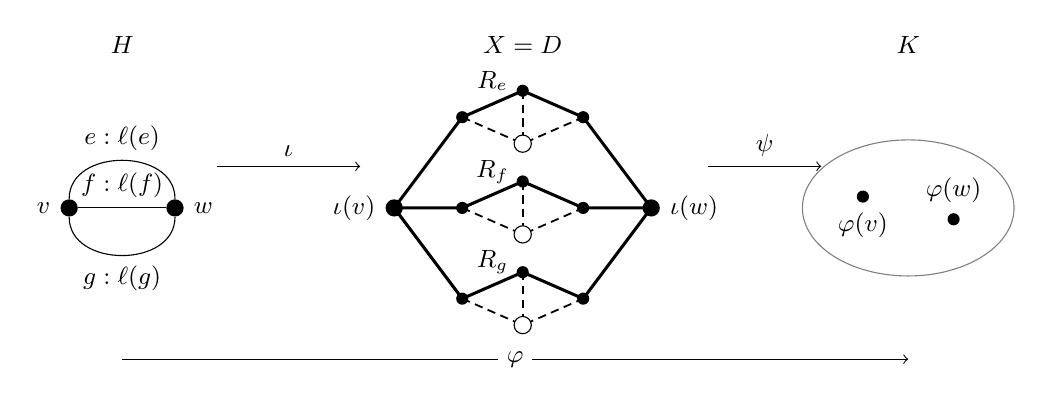
\begin{tikzpicture}[
  x=.96cm,y=.96cm,
  every node/.style={font=\small},
  vertex/.style={circle,fill=black,inner sep=1.55pt},
  branch/.style={circle,fill=black,inner sep=2.2pt},
  outside/.style={circle,draw=black,fill=white,inner sep=2.2pt},
  route/.style={line width=1.1pt},
  perron/.style={densely dashed,line width=.65pt},
]
\node at (0,2.15) {$H$};
\node at (5.3,2.15) {$X=D$};
\node at (10.4,2.15) {$K$};
\node[branch,label=left:$v$] (hu) at (-.7,0) {};
\node[branch,label=right:$w$] (hv) at (.7,0) {};
\draw (hu) .. controls (-.7,.8) and (.7,.8) .. (hv)
  node[midway,above] {$e:\ell(e)$};
\draw (hu)--(hv) node[midway,above] {$f:\ell(f)$};
\draw (hu) .. controls (-.7,-.8) and (.7,-.8) .. (hv)
  node[midway,below] {$g:\ell(g)$};

\coordinate (xu) at (3.6,0);
\coordinate (xv) at (7,0);
\foreach \height/\j in {1.2/e,0/f,-1.2/g} {
  \coordinate (a\j) at (4.5,\height);
  \coordinate (b\j) at (6.1,\height);
  \coordinate (c\j) at (5.3,\height+.35);
  \coordinate (d\j) at (5.3,\height-.35);
  \draw[perron] (a\j)--(d\j)--(b\j);
  \draw[perron] (c\j)--(d\j);
  \draw[route] (xu)--(a\j)--(c\j)--(b\j)--(xv);
  \foreach \p in {a,b,c} {\node[vertex] at (\p\j) {};}
  \node[outside] at (d\j) {};
  \node at (4.9,\height+.48) {$R_\j$};
}
\node[branch,label=left:$\iota(v)$] at (xu) {};
\node[branch,label=right:$\iota(w)$] at (xv) {};

\draw[black!50] (10.4,0) ellipse (1.4 and .9);
\node[vertex,label=below:$\varphi(v)$] at (9.8,.15) {};
\node[vertex,label=above:$\varphi(w)$] at (11,-.15) {};
\draw[->] (1.25,.55)--(3.15,.55) node[midway,above] {$\iota$};
\draw[->] (7.75,.55)--(9.25,.55) node[midway,above] {$\psi$};
\draw[->] (0,-2)--(10.4,-2)
  node[midway,fill=white,inner sep=3pt] {$\varphi$};
\end{tikzpicture}
\caption{The objects in \cref{lem:perron-transfer}, using $D$ from
\cref{fig:diamond-objects}.
Edges of $R_e$ have label $\ell(e)$; each solid path has three internal vertices.
Dashed edges have label $\rho_K$; hollow vertices lie outside all $R_e$.
The target $K$ is schematic, with two vertex images marked.
The coefficient $c_K(X,\ell_X)$ sums over all maps $\psi:V(X)\to V(K)$;
the right side of \cref{eq:perron-transfer} sums over all
$\varphi:V(H)\to V(K)$.
For a fixed $\psi$, we have $\varphi=\psi\circ\iota$.}
\label{fig:perron-objects}
\end{figure}

\begin{proof}
The vertices of $X$ consist of $\iota(V(H))$, the internal vertices of
the paths $R_e$, and the vertices outside all $R_e$.
Since $H$ and $X$ are cubic, the paths occupy all three edge incidences
at every vertex of $\iota(V(H))$. At an internal vertex of $R_e$, two incidences
belong to $R_e$; the third belongs to no chosen path, since their
interiors are disjoint. Every edge incident with a vertex outside all
$R_e$ lies outside the chosen subdivision.

In the sum defining $c_K(X,\ell_X)$, let $\psi:V(X)\to V(K)$ denote
the vertex map and put $\varphi=\psi\circ\iota$.
For each edge $vw$ outside all $R_e$, factor its projector entry as
$P_{\rho_K,K}(\psi(v),\psi(w))=u_K(\psi(v))u_K(\psi(w))$.
Regrouping these factors by their endpoints gives no $u_K$ factor
at vertices of $\iota(V(H))$, one at each internal path vertex, and three at each
vertex outside all $R_e$.
On the paths $R_e$, retain the projector factors $P_{\ell(e),K}$,
including when $\ell(e)=\rho_K$.
Summing over the image of each vertex outside all $R_e$ gives
$\sum_{x\in V(K)}u_K(x)^3=\tau_K$.
There are $|V(X)|-|V(H)|-\sum_eq_e$ such vertices.

For each edge $e=vw$, let $\lambda=\ell(e)$.
Summing over the image of one internal path vertex between fixed
neighbour images $x,y\in V(K)$ gives
\begin{equation}\label{eq:perron-path-factor}
 \sum_{z\in V(K)}P_{\lambda,K}(x,z)u_K(z)P_{\lambda,K}(z,y)
 =M_{\lambda,K}(x,y).
\end{equation}
Let $x_1,\ldots,x_{q_e}$ be the images of the internal vertices of $R_e$,
and put $x_0=\varphi(v)$ and $x_{q_e+1}=\varphi(w)$.
Since $P_{\lambda,K}^2=P_{\lambda,K}$ and $q_e\geq1$, summing over
these images gives
\begin{equation}\label{eq:path-image-sum}
 \sum_{x_1,\ldots,x_{q_e}\in V(K)}
 \left(\prod_{j=0}^{q_e}P_{\lambda,K}(x_j,x_{j+1})\right)
 \left(\prod_{j=1}^{q_e}u_K(x_j)\right)
 =M_{\lambda,K}^{q_e}(\varphi(v),\varphi(w)).
\end{equation}
For a loop $e$, we have $\varphi(v)=\varphi(w)$, so the same calculation gives a diagonal
entry of $M_{\lambda,K}^{q_e}$.
Summing over $\varphi$ now gives
\begin{equation}\label{eq:component-path-sum}
 c_K(X,\ell_X)
 =\tau_K^{|V(X)|-|V(H)|-\sum_eq_e}
   \sum_{\varphi:V(H)\to V(K)}
   \prod_{e=vw\in E(H)}M_{\ell(e),K}^{q_e}(\varphi(v),\varphi(w)).
\end{equation}
Substituting
$M_{\ell(e),K}^{q_e}=\tau_K^{q_e}(M_{\ell(e),K}/\tau_K)^{q_e}$
in \cref{eq:component-path-sum} proves \cref{eq:perron-transfer}.
The total exponent of $\tau_K$ is $|V(X)|-|V(H)|$, independent of the path lengths.
\end{proof}

\begin{lemma}\label{lem:positive-interpolation}
 Let $M_1,\ldots,M_p$ be positive semidefinite operators on finite-dimensional
 Euclidean spaces, and let $P_i$ be the orthogonal projector onto $\im M_i$.
 Suppose their spectra together contain at most $s$ distinct positive values,
 and let $Q$ be a set of at least $s$ distinct positive integers.
 Then there are coefficients $(a_q)_{q\in Q}$, only finitely many nonzero,
 with $\sum_{q\in Q}a_qM_i^q=P_i$ for every $i$.
\end{lemma}
\begin{proof}
 Let $\mu_1,\ldots,\mu_{s'}$ be the distinct positive
 values in the spectra of $M_1,\ldots,M_p$.
 Since $s'\leq s$, we can choose distinct elements $q_1,\ldots,q_{s'}$ of $Q$.
 The generalised Vandermonde matrix $(\mu_h^{q_j})_{h,j=1}^{s'}$ is
 invertible~\cite[p.~76]{GantmacherKrein2002}.
 Hence there are coefficients $a_{q_1},\ldots,a_{q_{s'}}$ with
 $\sum_ja_{q_j}\mu_h^{q_j}=1$ for every $h$; the remaining $a_q$ are zero.
 The operator $\sum_{q\in Q}a_qM_i^q$ is the identity on each positive
 eigenspace and is zero on $\ker M_i$, since every $q$ is positive.
 It therefore equals $P_i$.
\end{proof}

The next lemma combines two interpolations: one replaces operator powers
by image projectors, and the other removes scalar weights.
\begin{lemma}\label{lem:two-stage-interpolation}
 Let $\mathcal I,\mathcal J$ be finite sets. For each $i\in\mathcal I$ and $j\in\mathcal J$, let
 $M_{i,j}$ be a positive semidefinite operator on a finite-dimensional
 Euclidean space $V_{i,j}$, and let $P_{i,j}$ be the orthogonal projector
 onto $\im M_{i,j}$. Let $\Phi_i$ be a multilinear form on
 $\prod_{j\in\mathcal J}\operatorname{End}(V_{i,j})$, and let
 $\tau_i>0$ and $\varepsilon_i\in\R$.
 Let $(d_N)$ be an unbounded sequence of nonnegative integers.
 Suppose that, for every sufficiently large $N$, there are finite
 sets $Q_{N,j}\subseteq\Z_{\geq1}$ with
 $|Q_{N,j}|\geq\sum_{i\in\mathcal I}\dim V_{i,j}$,
 such that
 \begin{equation}\label{eq:two-stage-samples}
  \sum_{i\in\mathcal I}\varepsilon_i\tau_i^{d_N}
     \Phi_i((M_{i,j}^{q_j})_{j\in\mathcal J})=0
  \quad\text{for every }\mathbf q\in\prod_{j\in\mathcal J}Q_{N,j}.
 \end{equation}
 Then $\sum_{i\in\mathcal I}\varepsilon_i\Phi_i((P_{i,j})_{j\in\mathcal J})=0$.
\end{lemma}
\begin{proof}
 For each $j\in\mathcal J$, the spectra of the operators $(M_{i,j})_{i\in\mathcal I}$
 together contain at most $\sum_{i\in\mathcal I}\dim V_{i,j}$ distinct positive
 values. Thus, for each sufficiently large $N$ and each $j$,
 \cref{lem:positive-interpolation} gives coefficients $a_{N,j,q}$ with
 $\sum_{q\in Q_{N,j}}a_{N,j,q}M_{i,j}^q=P_{i,j}$ for every $i$.
 By multilinearity,
 \begin{equation}\label{eq:two-stage-operators}
  \sum_i\varepsilon_i\tau_i^{d_N}\Phi_i((P_{i,j})_j)
  =\sum_{\mathbf q\in\prod_jQ_{N,j}}
      \left(\prod_ja_{N,j,q_j}\right)
      \sum_i\varepsilon_i\tau_i^{d_N}\Phi_i((M_{i,j}^{q_j})_j)=0.
 \end{equation}
 Since $d_N$ is unbounded, we can choose $|\mathcal I|$ sufficiently large indices $N_h$
 with distinct positive values of $d_{N_h}$.
 Applying \cref{lem:positive-interpolation} to the operators
 $t\mapsto\tau_i t$ on $\R$ with these exponents gives coefficients $b_h$
 with $\sum_hb_h\tau_i^{d_{N_h}}=1$ for every $i$.
 Summing \cref{eq:two-stage-operators} at these indices with
 coefficients $b_h$ proves the lemma.
\end{proof}

\begin{lemma}\label{lem:cubic-coefficient-transfer}
 Let $(H_N)_{N\geq1}$ be a sequence of connected cubic graphs such that
 $H_N$ contains $K_{3N}$ as a minor for every $N\geq1$.
 Let $G,G'$ be finite simple graphs. Suppose
 $c_G(H_N,\ell)=c_{G'}(H_N,\ell)$ for every $N\geq1$ and every
 labelling $\ell:E(H_N)\to\R^\times$.
 Then $c_G(H,\ell)=c_{G'}(H,\ell)$ for every connected cubic
 multigraph $H$ and every labelling $\ell:E(H)\to\R^\times$.
\end{lemma}
\begin{proof}
For every graph $G$, connected multigraph $H$ with an edge, and nonzero
edge labelling $\ell$, we have
\begin{equation}\label{eq:component-contributions}
 c_G(H,\ell)=\sum_K c_K(H,\ell),
\end{equation}
where $K$ ranges over the connected components of $G$.
Indeed, the spectral projectors of $A_G$ are block diagonal over these
components, so a map $V(H)\to V(G)$ contributes zero unless its image
lies in one component.
For a component $K$, a label $\lambda>\rho_K$ on any edge gives
$c_K(H,\ell)=0$, because $P_{\lambda,K}=0$.

Fix an integer $n\geq0$. We prove the lemma for all pairs $G,G'$ with
$|V(G)|+|V(G')|\leq2n$.
The combined vertex bound allows the two graphs to have different
numbers of vertices after components are deleted.
We argue by induction on the total number of components containing an edge.
If both graphs are edgeless, including when either has no vertices,
every labelled coefficient of a connected cubic multigraph is zero.
Otherwise $n\geq1$. Let $r>0$ be the largest spectral radius among all
components of both graphs, and let $\mathcal K,\mathcal K'$ consist of
the components of $G,G'$, respectively, with spectral radius $r$.
Since $r$ is attained, $\mathcal K\sqcup\mathcal K'\ne\varnothing$.
Fix a connected cubic multigraph $H$ and a nonzero edge labelling $\ell$.
We prove that
\begin{equation}\label{eq:layer-contractions}
 \sum_{K\in\mathcal K}c_K(H,\ell)
 =\sum_{K\in\mathcal K'}c_K(H,\ell).
\end{equation}
Apply \cref{lem:independent-path-lengths} with $m=2n$ to obtain $D$.
For every sufficiently large $N$, \cref{lem:subdivision-containment}
places a subdivision of $D$ in $H_N$.
Hence \cref{lem:independent-path-lengths} supplies an injection
$\iota:V(H)\hookrightarrow V(H_N)$ and sets
$Q_e\subseteq\Z_{\geq1}$ with $|Q_e|\geq2n+1$.
For each $\mathbf q\in\prod_eQ_e$, choose the paths $R_e$ given by that
lemma. Let $\ell_N(\mathbf q)$ assign $\ell(e)$ to the edges of $R_e$
and $r$ to every edge outside the paths.
This is the labelling $\ell_X$ in \cref{lem:perron-transfer} with
$X=H_N$ and $\rho_K=r$.
At least one edge receives $r$, so only components in $\mathcal K$
contribute to $c_G(H_N,\ell_N(\mathbf q))$.
Put $n_N=|V(H_N)|$ and $n_H=|V(H)|$.
Since $\rho_K=r$ for every $K\in\mathcal K$, applying
\cref{lem:perron-transfer} to each such $K$ and using
\cref{eq:component-contributions} gives
\begin{equation}\label{eq:operator-transfer}
 c_G(H_N,\ell_N(\mathbf q))=\sum_{K\in\mathcal K}\tau_K^{n_N-n_H}
   \sum_{\varphi:V(H)\to V(K)}
   \prod_{e=vw\in E(H)}
       \left(\frac{M_{\ell(e),K}}{\tau_K}\right)^{q_e}(\varphi(v),\varphi(w)).
\end{equation}
The same labelling satisfies \cref{eq:operator-transfer} for $G'$ and
$\mathcal K'$ because every $K\in\mathcal K'$ also has $\rho_K=r$.
We suppress the dependence of the sets $Q_e$ on $N$.
Interpolation over $q_e$ in \cref{eq:operator-transfer} will replace
$(M_{\ell(e),K}/\tau_K)^{q_e}$ by $P_{\ell(e),K}$.
Interpolation over $N$ will then replace $\tau_K^{n_N-n_H}$ by $1$.

We apply \cref{lem:two-stage-interpolation} with component index set
$\mathcal I=\mathcal K\sqcup\mathcal K'$ and edge index set $\mathcal J=E(H)$.
The signs are $+1$ on $\mathcal K$ and $-1$ on $\mathcal K'$.
For each component $K$ and edge $e$, the operator is
$M_{\ell(e),K}/\tau_K$ on $\R^{V(K)}$.
It is positive semidefinite with image projector $P_{\ell(e),K}$.
For each component $K$, let
\begin{equation}\label{eq:component-multilinear-form}
 \Phi_K((T_e)_{e\in E(H)})
 =\sum_{\varphi:V(H)\to V(K)}
   \prod_{e=vw\in E(H)}T_e(\varphi(v),\varphi(w)),
\end{equation}
where each $T_e$ is a matrix indexed by $V(K)$.
This form is multilinear, and $\Phi_K((P_{\ell(e),K})_e)=c_K(H,\ell)$.
The spaces $\R^{V(K)}$ have total dimension
$\sum_{K\in\mathcal K\sqcup\mathcal K'}|V(K)|\leq2n$.
Every $Q_e$ has at least $2n+1$ elements, so the dimension bound
in \cref{lem:two-stage-interpolation} holds.
The assumed equality of the two instances of \cref{eq:operator-transfer}
is exactly \cref{eq:two-stage-samples} with $d_N=n_N-n_H$.
Since $H_N$ contains a $K_{3N}$ minor, $n_N\geq3N$.
Thus $d_N$ is nonnegative for all sufficiently large $N$ and is unbounded.
Hence \cref{lem:two-stage-interpolation} proves \cref{eq:layer-contractions}.

Let $G^-$ and $G'^-$ be obtained by deleting the components in
$\mathcal K$ and $\mathcal K'$, respectively.
Let $N_\ast\geq1$ and let $\eta$ be a nonzero labelling of $H_{N_\ast}$.
Since $H_{N_\ast}$ is connected and cubic, \cref{eq:layer-contractions} holds
with $H=H_{N_\ast}$ and $\ell=\eta$, so by \cref{eq:component-contributions}
and the assumed equality on $H_{N_\ast}$,
\begin{equation}\label{eq:residual-contractions}
 \begin{aligned}
 c_{G^-}(H_{N_\ast},\eta)
 &=c_G(H_{N_\ast},\eta)-\sum_{K\in\mathcal K}c_K(H_{N_\ast},\eta)\\
 &=c_{G'}(H_{N_\ast},\eta)-\sum_{K\in\mathcal K'}c_K(H_{N_\ast},\eta)
 =c_{G'^-}(H_{N_\ast},\eta).
 \end{aligned}
\end{equation}
We have $|V(G^-)|+|V(G'^-)|\leq2n$.
Since $\mathcal K\sqcup\mathcal K'\ne\varnothing$ and $r>0$, deleting
these components strictly decreases the total number containing an edge.
The induction hypothesis therefore gives
$c_{G^-}(H,\ell)=c_{G'^-}(H,\ell)$ for every connected cubic $H$ and
nonzero labelling $\ell$.
Adding the equal sums in \cref{eq:layer-contractions} and using
\cref{eq:component-contributions} gives $c_G(H,\ell)=c_{G'}(H,\ell)$,
proving the lemma.
\end{proof}

\begin{proof}[Proof of \cref{prop:closure}]
By the initial reduction, it suffices to prove the equivalence for $\calF'$.
Suppose $G\equiv_{\calF'}G'$. Since $K_1\in\calF'$, we have
$|V(G)|=|V(G')|$.
Their counts agree on every subdivision $H_N^{\mathbf m}$.
By \cref{lem:subdivision-coefficients},
$c_G(H_N,\ell)=c_{G'}(H_N,\ell)$ for every $N$ and every nonzero labelling $\ell$.
\Cref{lem:cubic-coefficient-transfer} therefore gives equality of the labelled
coefficients on every connected cubic multigraph. By \cref{lem:characterisation}(c),
$G\equiv_{\mathcal D_3}G'$.
The reverse implication follows from $\calF'\subseteq\mathcal D_3$,
and completeness on simple spectrum follows from \cref{thm:main}.
\end{proof}


\section*{Declarations}

The author used OpenAI GPT-6 Astra and Anthropic Claude Opus 5.5 in
preparing this work. The author formulated the problem and initial
theorem statements. GPT-6 Astra assisted with mathematical exploration
and identifying relevant literature. The proofs were developed through
discussions between the author and GPT-6 Astra. GPT-6 Astra and Claude
Opus 5.5 both assisted with checking readability and improving the
presentation. The author assumes responsibility for all content.

\bibliographystyle{plain}
\bibliography{references}
\end{document}
